\documentclass[cjk,dvipdfmx,10pt,compress,fragile%
hyperref={bookmarks=true,bookmarksnumbered=true,bookmarksopen=false,%
colorlinks=false,%
pdftitle={第 134 回 関西 Debian 勉強会},%
pdfauthor={小林},%
%pdfinstitute={関西 Debian 勉強会},%
pdfsubject={資料},%
}]{beamer}

\title{自作キーボード温泉に日帰り入浴してみた話}
\author[Katsuki Kobayashi]{{\large\bf Katsuki Kobayashi}}
\institute[Debian JP]{{\normalsize\tt 関西 Debian 勉強会}}
\date{{\small 2019年 11月 24日 (日)}}

\usepackage{graphicx}
\usepackage{moreverb}
\usepackage{ulem}
\usepackage[varg]{txfonts}
\usepackage{tabularx}
\usepackage{fancybox}
\usepackage{fancyvrb}
\usepackage{float}
\usepackage{multicol}
\usepackage{minijs}
\usepackage{amsmath}
\usepackage{amssymb}
\usepackage{newtxtext}
\usepackage{listings}
\usepackage{xcolor}
\usepackage{hyperref}
\AtBeginDvi{\special{pdf:tounicode EUC-UCS2}}
\usetheme{KansaiDebian}
\def\museincludegraphics{%
  \begingroup
  \catcode`\|=0
  \catcode`\\=12
  \catcode`\#=12
  \includegraphics[width=0.9\textwidth]}
%\renewcommand{\familydefault}{\sfdefault}
%\renewcommand{\kanjifamilydefault}{\sfdefault}
%
\newenvironment{commandline}%
{\VerbatimEnvironment
  \begin{Sbox}\begin{minipage}{0.9\hsize}\begin{fontsize}{8}{8} \color{white} \begin{BVerbatim}}%
{\end{BVerbatim}\end{fontsize}\end{minipage}\end{Sbox}
  \setlength{\fboxsep}{8pt}
% start on a new paragraph

\vspace{6pt}% skip before
\fcolorbox{white}{black}{\TheSbox}

\vspace{3pt}% skip after
}
%end of commandline

\newenvironment{tinycommandline}%
{\VerbatimEnvironment
  \begin{Sbox}\begin{minipage}{0.9\hsize}\begin{fontsize}{4}{4} \color{white} \begin{BVerbatim}}%
{\end{BVerbatim}\end{fontsize}\end{minipage}\end{Sbox}
  \setlength{\fboxsep}{8pt}
% start on a new paragraph

\vspace{6pt}% skip before
\fcolorbox{white}{black}{\TheSbox}

\vspace{3pt}% skip after
}
%end of tinycommandline

\begin{document}

\begin{frame}[fragile]
\titlepage
\end{frame}

\begin{frame}[fragile,t]{お詫び}
 \begin{itemize}
  \item Debian要素はあんまりないです
 \end{itemize}
\end{frame}

\takahashi[40]{みなさん}
\takahashi[40]{肩や腰は\\大丈夫ですか?}
\takahashi[40]{私は駄目です}

\begin{frame}[fragile,t]{自作キーボードへの動機(1/4)}
 \begin{itemize}
  \item 会社にて腰痛が酷くて、対策しても効果がない
	\begin{itemize}
	 \item 整骨院に通う
	 \item ジムで筋トレする
	\end{itemize}
  \item 特に、ここ数年酷い
	\pause
  \item 心当たり
 \end{itemize}
\begin{center}
 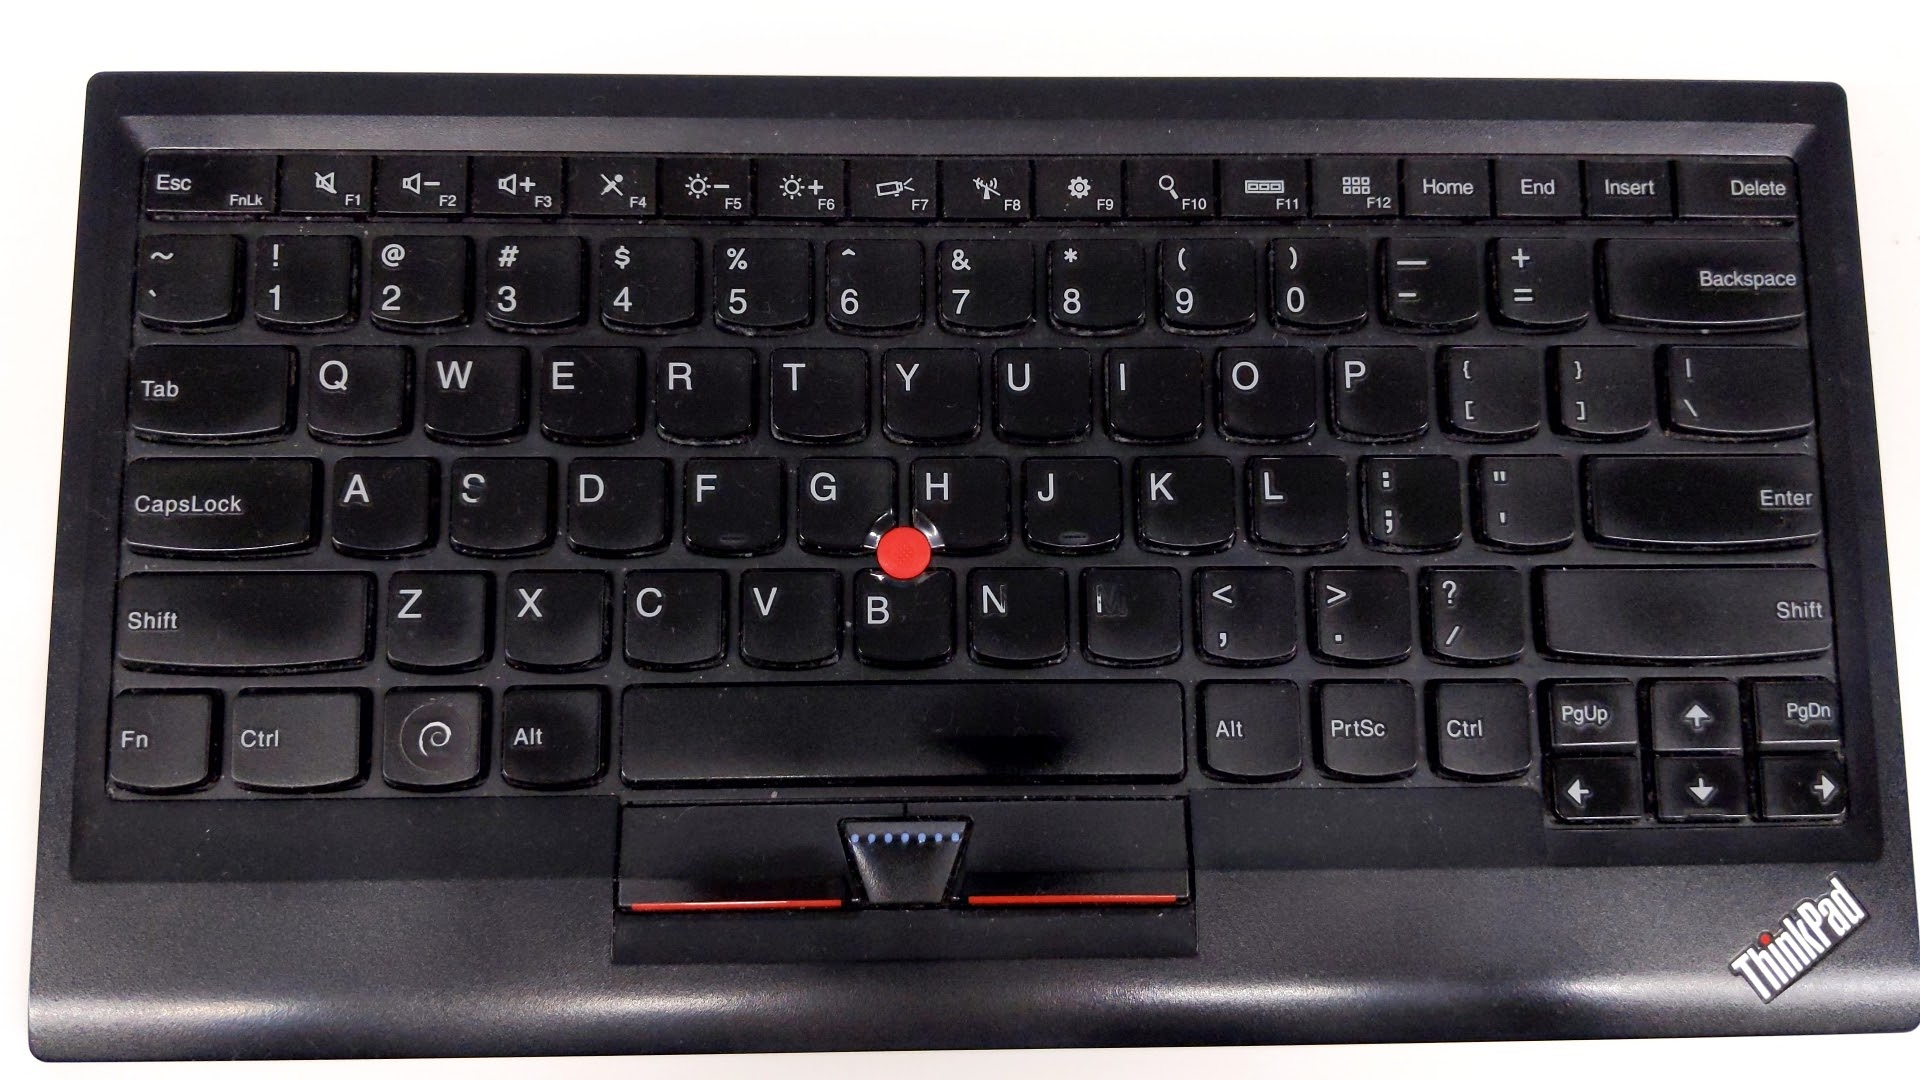
\includegraphics[keepaspectratio,height=4cm]{./img/thinkpad_kb.jpg}
\end{center}
\end{frame}

\begin{frame}[fragile,t]{自作キーボードへの動機(2/4)}
 \begin{itemize}
  \item ThinkPadキーボード
	\begin{itemize}
	 \item ThinkPadを使い始めて約4年
	 \item トラックポイントの良さに気付いて会社でもThinkPadキーボードに
	       \begin{itemize}
		\item WindowsではLinuxほど恩恵には預かれないけど
	       \end{itemize}
	 \item トラックポイントが悪いのかと思い、ここ数ヶ月はマウスを使用
	       \begin{itemize}
		\item しかし改善せず……
	       \end{itemize}
	\end{itemize}
	\pause
  \item 分割型キーボード
	\begin{itemize}
	 \item まぁ、肩凝りには効きそう
	 \item しかし、腰に効くのか想像できない
	\end{itemize}
 \end{itemize}
\end{frame}

\begin{frame}[fragile,t]{自作キーボードへの動機(3/4)}
 \begin{itemize}
  \item \href{https://ultimatehackingkeyboard.com/}{Ultimate Hacking Keyboard}なるものをみつける
	\begin{itemize}
	 \item トラックポイントが付く!!
	       \begin{itemize}
		\item しかし場所がおかしい
		\item トラックボールやタッチパッドも付けられる
	       \end{itemize}
	 \item 軸は変更できる
	       \begin{itemize}
		\item 軸については後ほど……
	       \end{itemize}
	 \item ファームもカスタマイズできる
	 \item でもお値段的に
	       \begin{itemize}
		\item 最小構成でも275ドル
		\item トラックポイントつけたり、レストアームつけると4万円越え
		\item 海外なので、送料やら納期がなぁ……
	       \end{itemize}
	\end{itemize}
 \end{itemize}
\end{frame}

\begin{frame}[fragile,t]{自作キーボードへの動機(4/4)}
 \begin{itemize}
  \item 沼の住人からお声かけいただく
	\begin{itemize}
	 \item \url{https://twitter.com/rarewin/status/1163656414184689665}
	\end{itemize}
  \item \href{https://mechanicalkeyboards.com/shop/index.php?l=product_detail&p=3532}{Tex Yoda II}
	\begin{itemize}
	 \item 分割されてたら求めていた感じだった
	\end{itemize}
  \item 自作キーボードにトラックポイントを付けている人は一定数いるらしい
	\begin{itemize}
	 \item \href{https://www.google.com/search?client=firefox-b-e&q=%E3%83%88%E3%83%A9%E3%83%83%E3%82%AF%E3%83%9D%E3%82%A4%E3%83%B3%E3%83%88+%E8%87%AA%E4%BD%9C%E3%82%AD%E3%83%BC%E3%83%9C%E3%83%BC%E3%83%89}{Google検索: トラックポイント 自作キーボード}
	\end{itemize}
  \item そんなこんなで、自作へと心が……
 \end{itemize}
\end{frame}

\begin{frame}[fragile,t]{キーボードの選定(1/2)}
 \begin{itemize}
  \item ということで自作してみる
	\begin{itemize}
	 \item 自分の追い求めた理想のキーボードを \textbf{Endgame} というそうです
	 \item そこまで深みにはまる気はないですけどね
	\end{itemize}
  \item 個人的に試したかったもの
	\begin{itemize}
	 \item 分割キーボード - 肩凝りに効きそうだったので必須
	 \item なるべく普通な配列 - 格子配列とかはひとまず避けたい
	 \item 打鍵音は静かなのがいい
	 \item 打鍵感も軽くてよい
	 \item トラックポイント欲しい……が、一旦あきらめる
	\end{itemize}
 \end{itemize}
\end{frame}

\begin{frame}[fragile,t]{キーボードの選定(2/2)}
 \begin{itemize}
  \item 考えるべき事はいくつかある
  \item 各キーの配列はファームウェアがあるのでなんとでもなる
	\begin{itemize}
	 \item QWERTY配列とDvorak配列を切り替えられるようなファームもある
	\end{itemize}
  \item キーの配置
	\begin{itemize}
	 \item 普通の
	 \item 格子状 -- 省スペース! (代表: \href{https://yushakobo.jp/shop/helix-keyboard-kit/}{Helix})
	 \item エルゴノミクス -- 指の長さや親指の稼動域を考慮 (代表: \href{ErgoDox}{https://ergodox-ez.com/})
	\end{itemize}
  \item キーの数
	\begin{itemize}
	 \item XX\%キーボード -- フルキー(104キー)に対して何個のキーがあるか
	       \begin{itemize}
		\item 主流は60\%くらい (数字キーの段あり、テンキー、FunctionKeyなし)
		\item さらにいくと40\%くらい (数字キーなし、カーソルキー、一部の記号キーがない)
		\item \href{https://www.reddit.com/r/MechanicalKeyboards/comments/dnrvz8/science_isnt_about_why_its_about_why_not/}{あたまおかしいの 10\%}
		\item 逆に100を越えるのも(ゲーム用とか)
	       \end{itemize}
	\end{itemize}
 \end{itemize}
\end{frame}

\begin{frame}[fragile,t]{一般的な自作キーボードキットの構成}
 \begin{itemize}
  \item 大体のキットについてくるもの
	\begin{itemize}
	 \item 基板 (基盤と書くと警察が来る)
	 \item マイコン -- 大体Promicro
	 \item プレート -- カバー
	 \item ダイオード -- キーマトリックス用
	 \item リセットスイッチ -- ファーム焼きのため
	 \item OLED(オプション)
	 \item LED(オプション)
	\end{itemize}
  \item 自分で用意する場合があるもの
	\begin{itemize}
	 \item キースイッチ
	 \item キーキャップ
	 \item ケーブル (USB/TRRS)
	\end{itemize}
 \end{itemize}
\end{frame}

\begin{frame}[fragile,t]{自作キット紹介 : Mint60}
 \begin{itemize}
  \item 私は一台目として購入 (\href{https://eucalyn.shop/shop/kits/mint60-starter}{公式販売サイト})
  \item オーソドックスな分割60\%キーボード
  \item キースイッチ/キャップ付きのキットがあって購入しやすい
	\begin{itemize}
	 \item スイッチ/キャップは数種類から選べる
	\end{itemize}
  \item 組み立ての難易度も低い
	\begin{itemize}
	 \item 半田付け難易度の高い素子(チップダイオード/チップLEDなど)はない
	 \onslide<2>{\item ただし、発表者は未だにシリアル通信が動いていない}
	\end{itemize}
  \item 作者の人は関西の人? (発送元が奈良だった)けど東京で精力的にイベント主催
	\begin{itemize}
	 \item \href{https://tenkey.connpass.com/event/150626/}{天下一キーボードわいわい会 Vol.3}
	 \item \href{https://connpass.com/event/149388/}{Mint60組み立て会 Vol.4}
	\end{itemize}
 \end{itemize}
 \begin{center}
  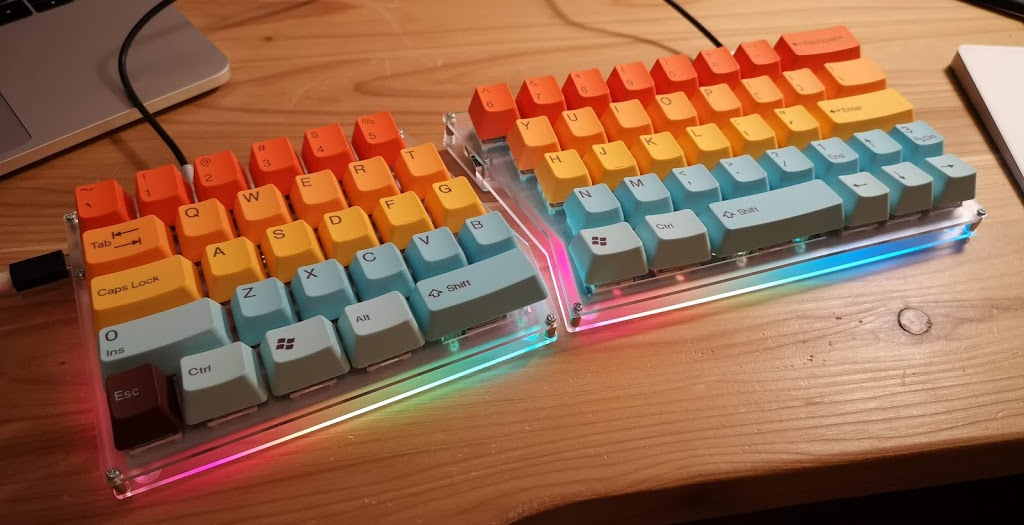
\includegraphics[keepaspectratio,height=1.5cm]{./img/mint60-hawaii.jpg}
  \hspace*{1zw}
  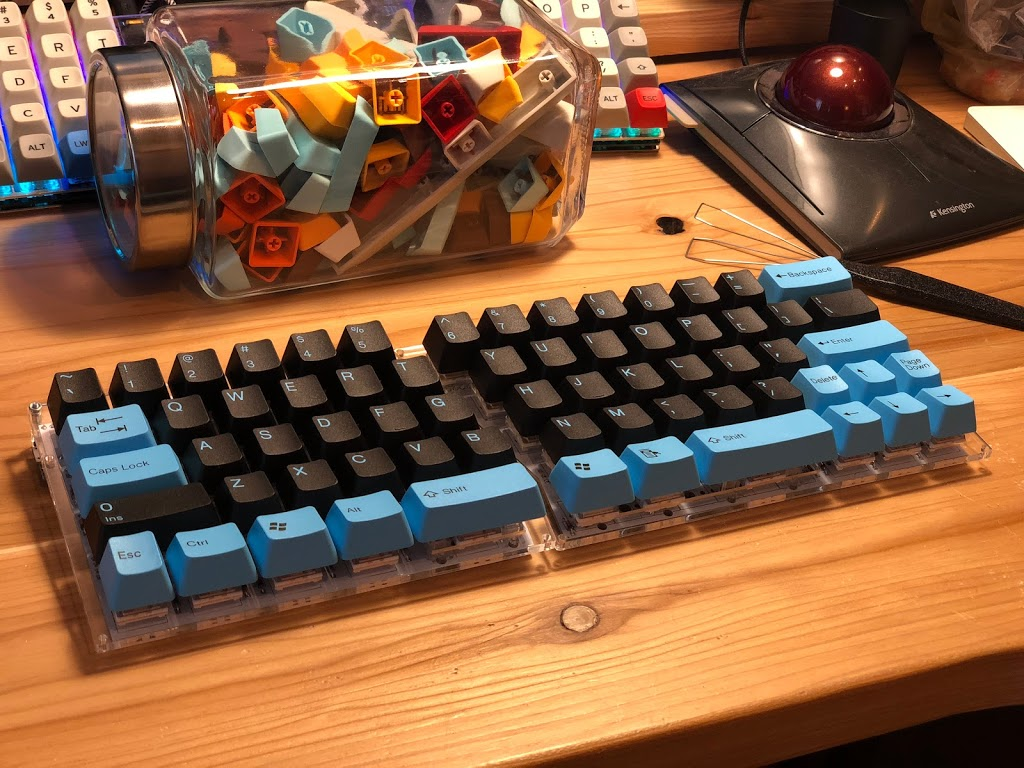
\includegraphics[keepaspectratio,height=1.5cm]{./img/mint60-starry-night.jpg}
  \hspace*{1zw}
  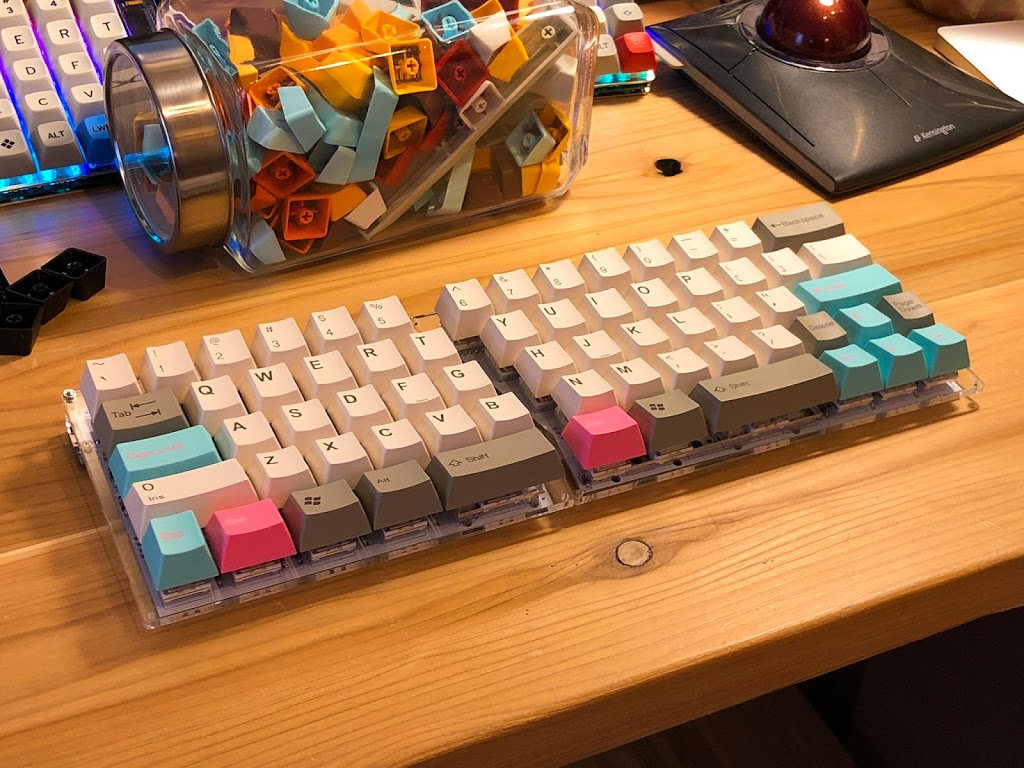
\includegraphics[keepaspectratio,height=1.5cm]{./img/mint60-miami-blue.jpg}
 \end{center}
 \vspace*{-1zw}
 \begin{flushright}
  {\footnotesize 引用元: \url{http://eucalyn.hatenadiary.jp/entry/about-mint60-01}}
 \end{flushright}
\end{frame}

\begin{frame}[fragile,t]{自作キット紹介 : Helix}
 \begin{itemize}
  \item 私はMint60の後にThinkpadの左手用として購入 (\href{https://yushakobo.jp/shop/helix-keyboard-kit/}{販売サイト})
  \item 遊舎工房の代表者の倉内さんが設計したキーボード
  \item 特徴的な完全な格子配列
	\begin{itemize}
	 \item キー数的には60\%くらい(64キー)、14キー減らすこともできる
	 \item PCBがリバーシブルなのでカーソル等の位置が特殊
	\end{itemize}
  \item 基板の設計がとても綺麗
	\begin{itemize}
	 \item Cherry/Kailhロープロファイル 両対応
	 \item ダイオードもチップ/素子両対応(キット付属はチップタイプ)
	\end{itemize}
  \item PCBのデータが公開されていて派生キーボードも多い
 \end{itemize}
 \begin{center}
  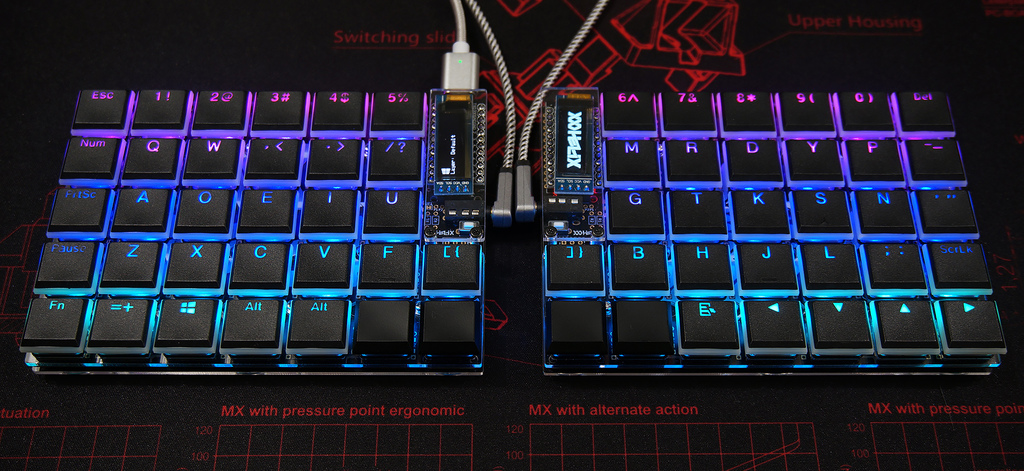
\includegraphics[keepaspectratio,height=1.5cm]{./img/helix-5rows-kailh.jpg}
  \hspace*{1zw}
  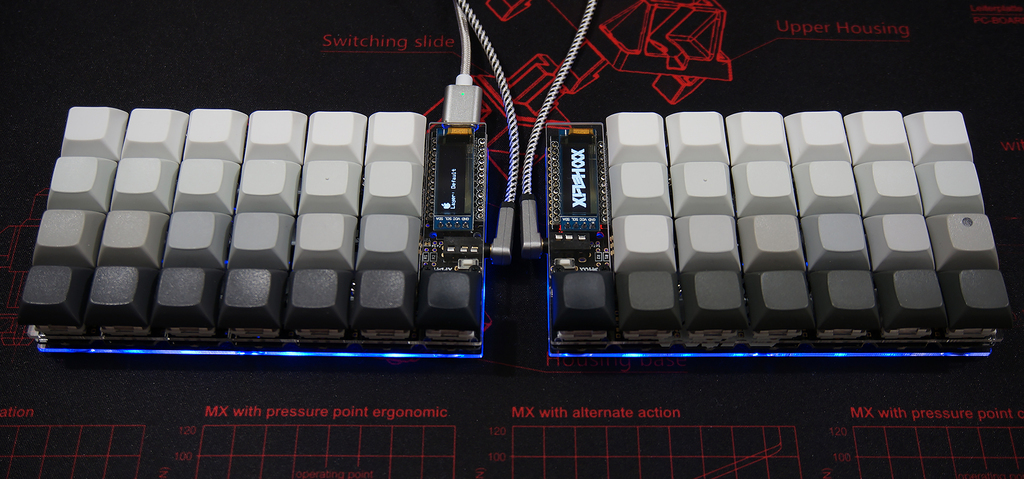
\includegraphics[keepaspectratio,height=1.5cm]{./img/helix-4rows-cherry.jpg}
  \hspace*{1zw}
  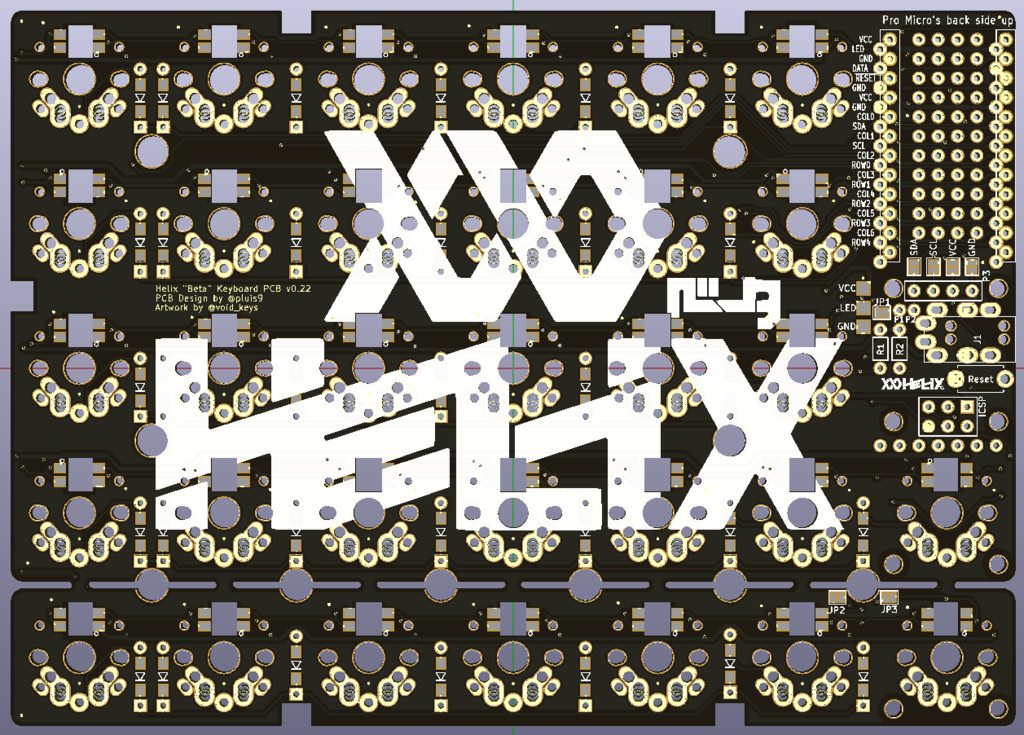
\includegraphics[keepaspectratio,height=1.5cm]{./img/helix-pcb.jpg}
 \end{center}
 \vspace*{-1zw}
 \begin{flushright}
  {\footnotesize 引用元: \url{https://yushakobo.jp/shop/helix-keyboard-kit/}}
 \end{flushright}
\end{frame}

\begin{frame}[fragile,t]{自作キット紹介 : Claw44}
 \begin{itemize}
  \item 会社の同僚が購入 (\href{https://yushakobo.jp/shop/consign_claw44/}{販売サイト})
  \item 配列が特徴的
	\begin{itemize}
	 \item 指の移動方向に合わせて設計
	 \item 特に親指がわかりやすそう
	\end{itemize}
  \item キーが相当に少ないので、同僚は諦め風味
 \end{itemize}
 \begin{center}
  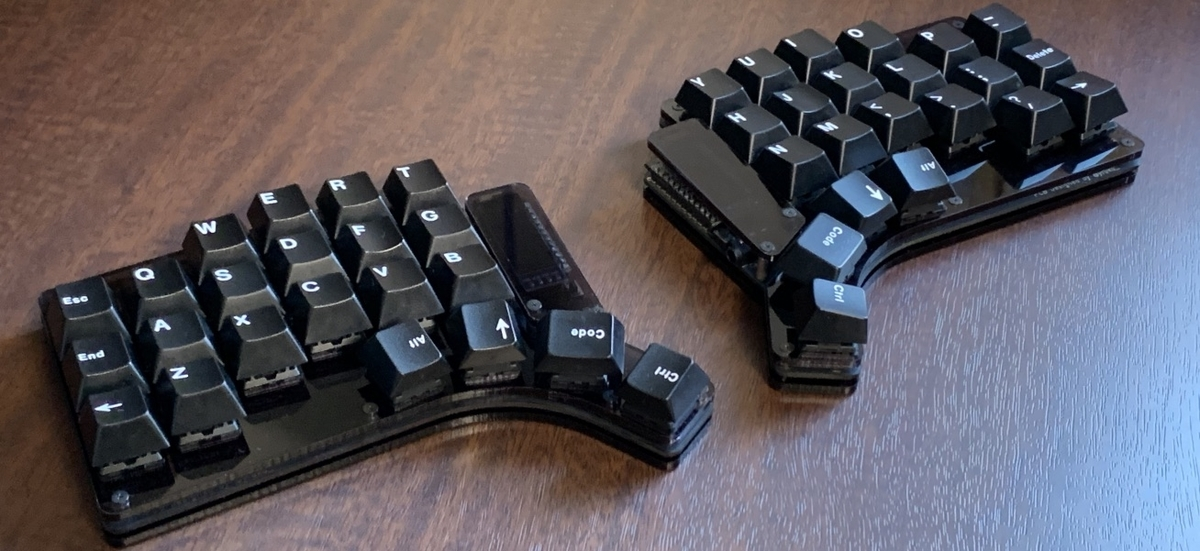
\includegraphics[keepaspectratio,height=2.5cm]{./img/claw44-01.jpg}
  \hspace*{1zw}
  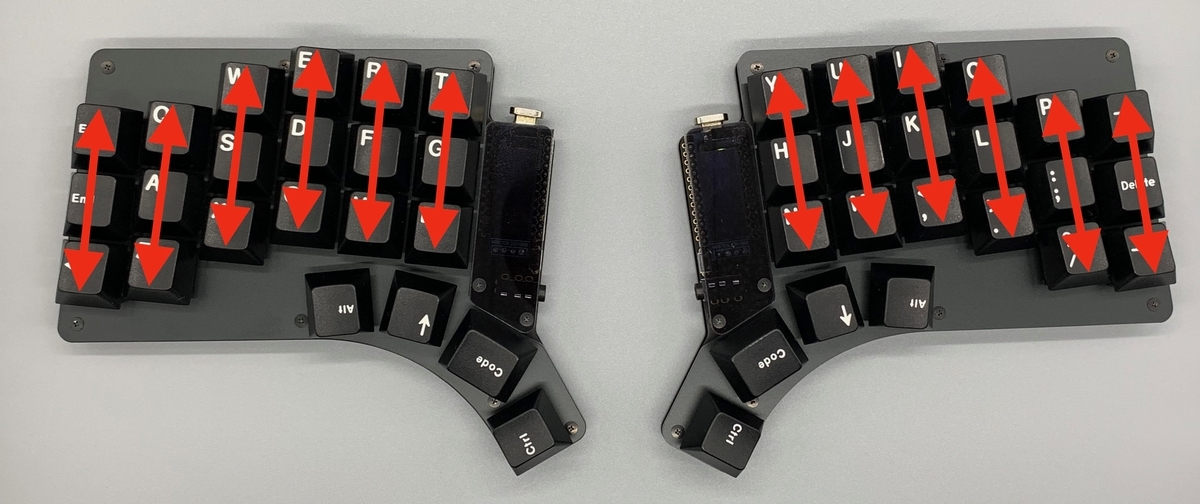
\includegraphics[keepaspectratio,height=2.5cm]{./img/claw44-02.jpg}
 \end{center}
 \vspace*{-1zw}
 \begin{flushright}
  {\footnotesize 引用元: \url{https://blog.yfuku.com/entry/claw44}}
 \end{flushright}
\end{frame}

\begin{frame}[fragile,t]{自作キット紹介 : Fortitude60}
 \begin{itemize}
  \item 名前が特徴的なキット (\href{https://yushakobo.jp/shop/fortitude60/}{販売サイト})
	\begin{itemize}
	 \item イキリホワイト
	 \item オタクブラック
	\end{itemize}
  \item promicroをつかっていない
  \item 貴重なUSB Type-C
	\begin{itemize}
	 \item Type-Cをつけたpromicroクローンも存在はしている(けど希少で割高)
	\end{itemize}
 \end{itemize}
 \begin{center}
  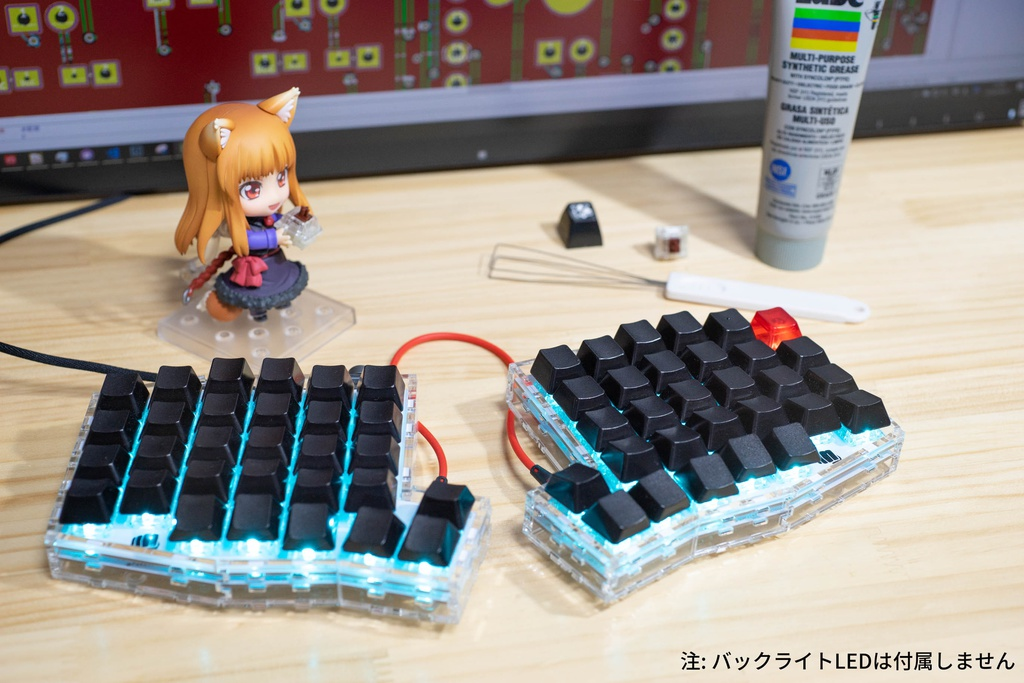
\includegraphics[keepaspectratio,height=2.5cm]{./img/fortitude60-ikiri.jpg}
  \hspace*{.5zw}
  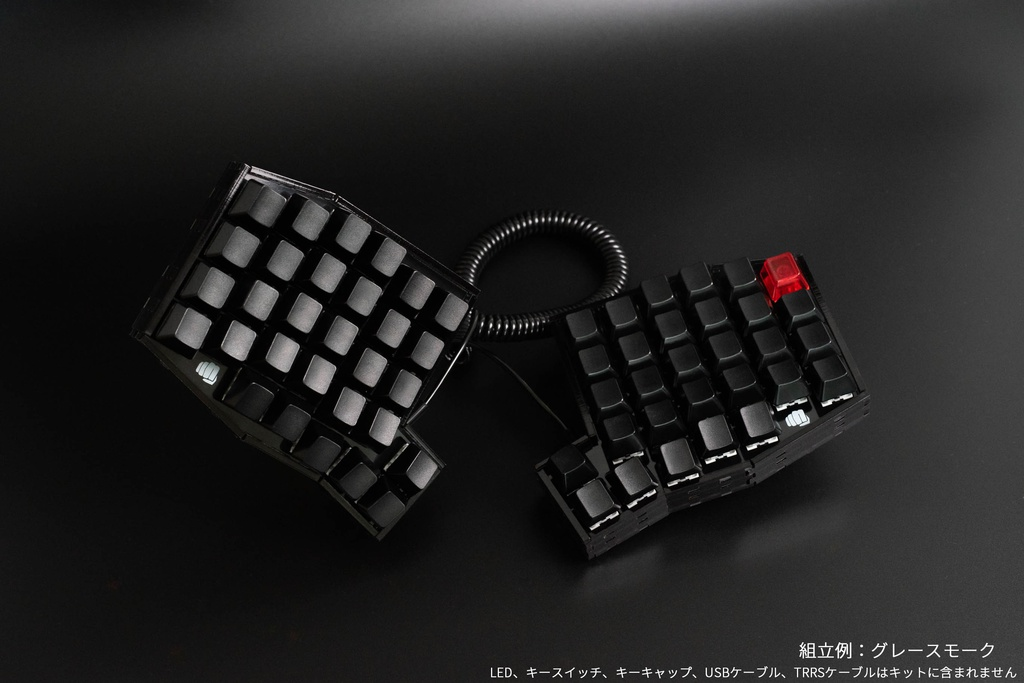
\includegraphics[keepaspectratio,height=2.5cm]{./img/fortitude60-otaku.jpg}
  \hspace*{.5zw}
  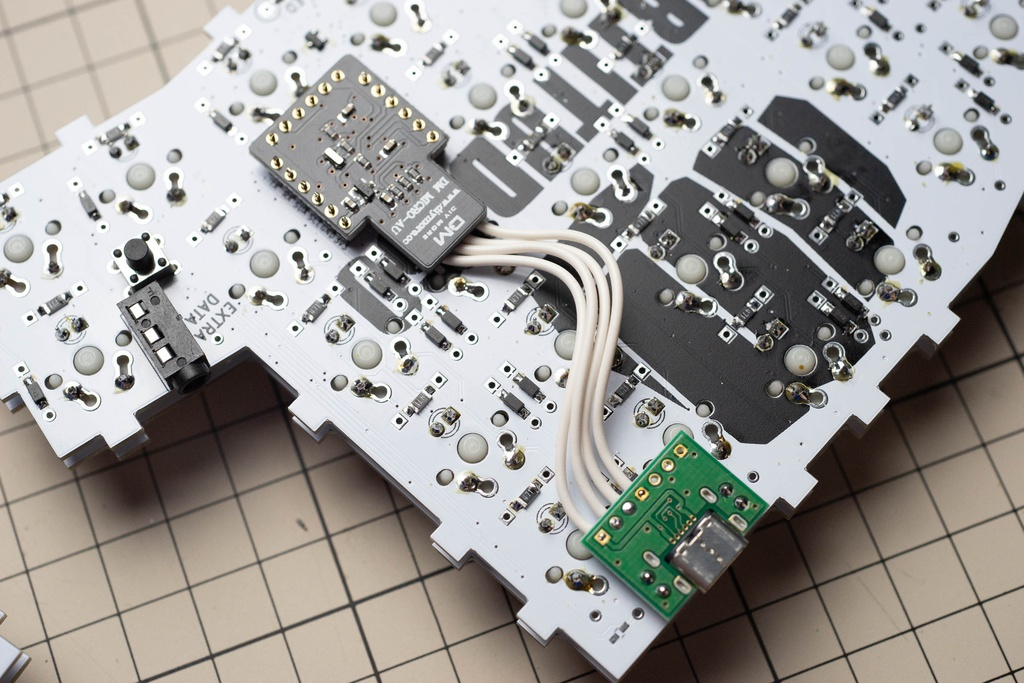
\includegraphics[keepaspectratio,height=2.5cm]{./img/fortitude60-typec.jpg}
 \end{center}
 \vspace*{-1zw}
 \begin{flushright}
  {\footnotesize
  引用元: \url{https://booth.pm/ja/items/1071554}}
 \end{flushright}
\end{frame}

\begin{frame}[fragile,t]{キースイッチ(1/3)}
 \begin{itemize}
  \item 現状、普及しているのは以下の2種類?
	\begin{itemize}
	 \item Cherry MX (左)  - ドイツCherry社
	       \begin{itemize}
		\item 特許が切れているためクローンがいっぱいある模様 (Gateron等)
		\item 出回っているキットはほとんど対応
		\item 最近ロープロファイルが出た? \href{https://www.cherrymx.de/en/mx-low-profile/mx-low-profile-red.html}{参考}
	       \end{itemize}
	 \item Kailh ロープロファイル (右) - 中国のKaihua?
	       \begin{itemize}
		\item Cherry MXとは互換性がない(対応している基板が必要)ので注意が必要
	       \end{itemize}
	\end{itemize}
  \item みなさんご存知の通り、色によって押し具合が変わる
 \end{itemize}
 \begin{center}
  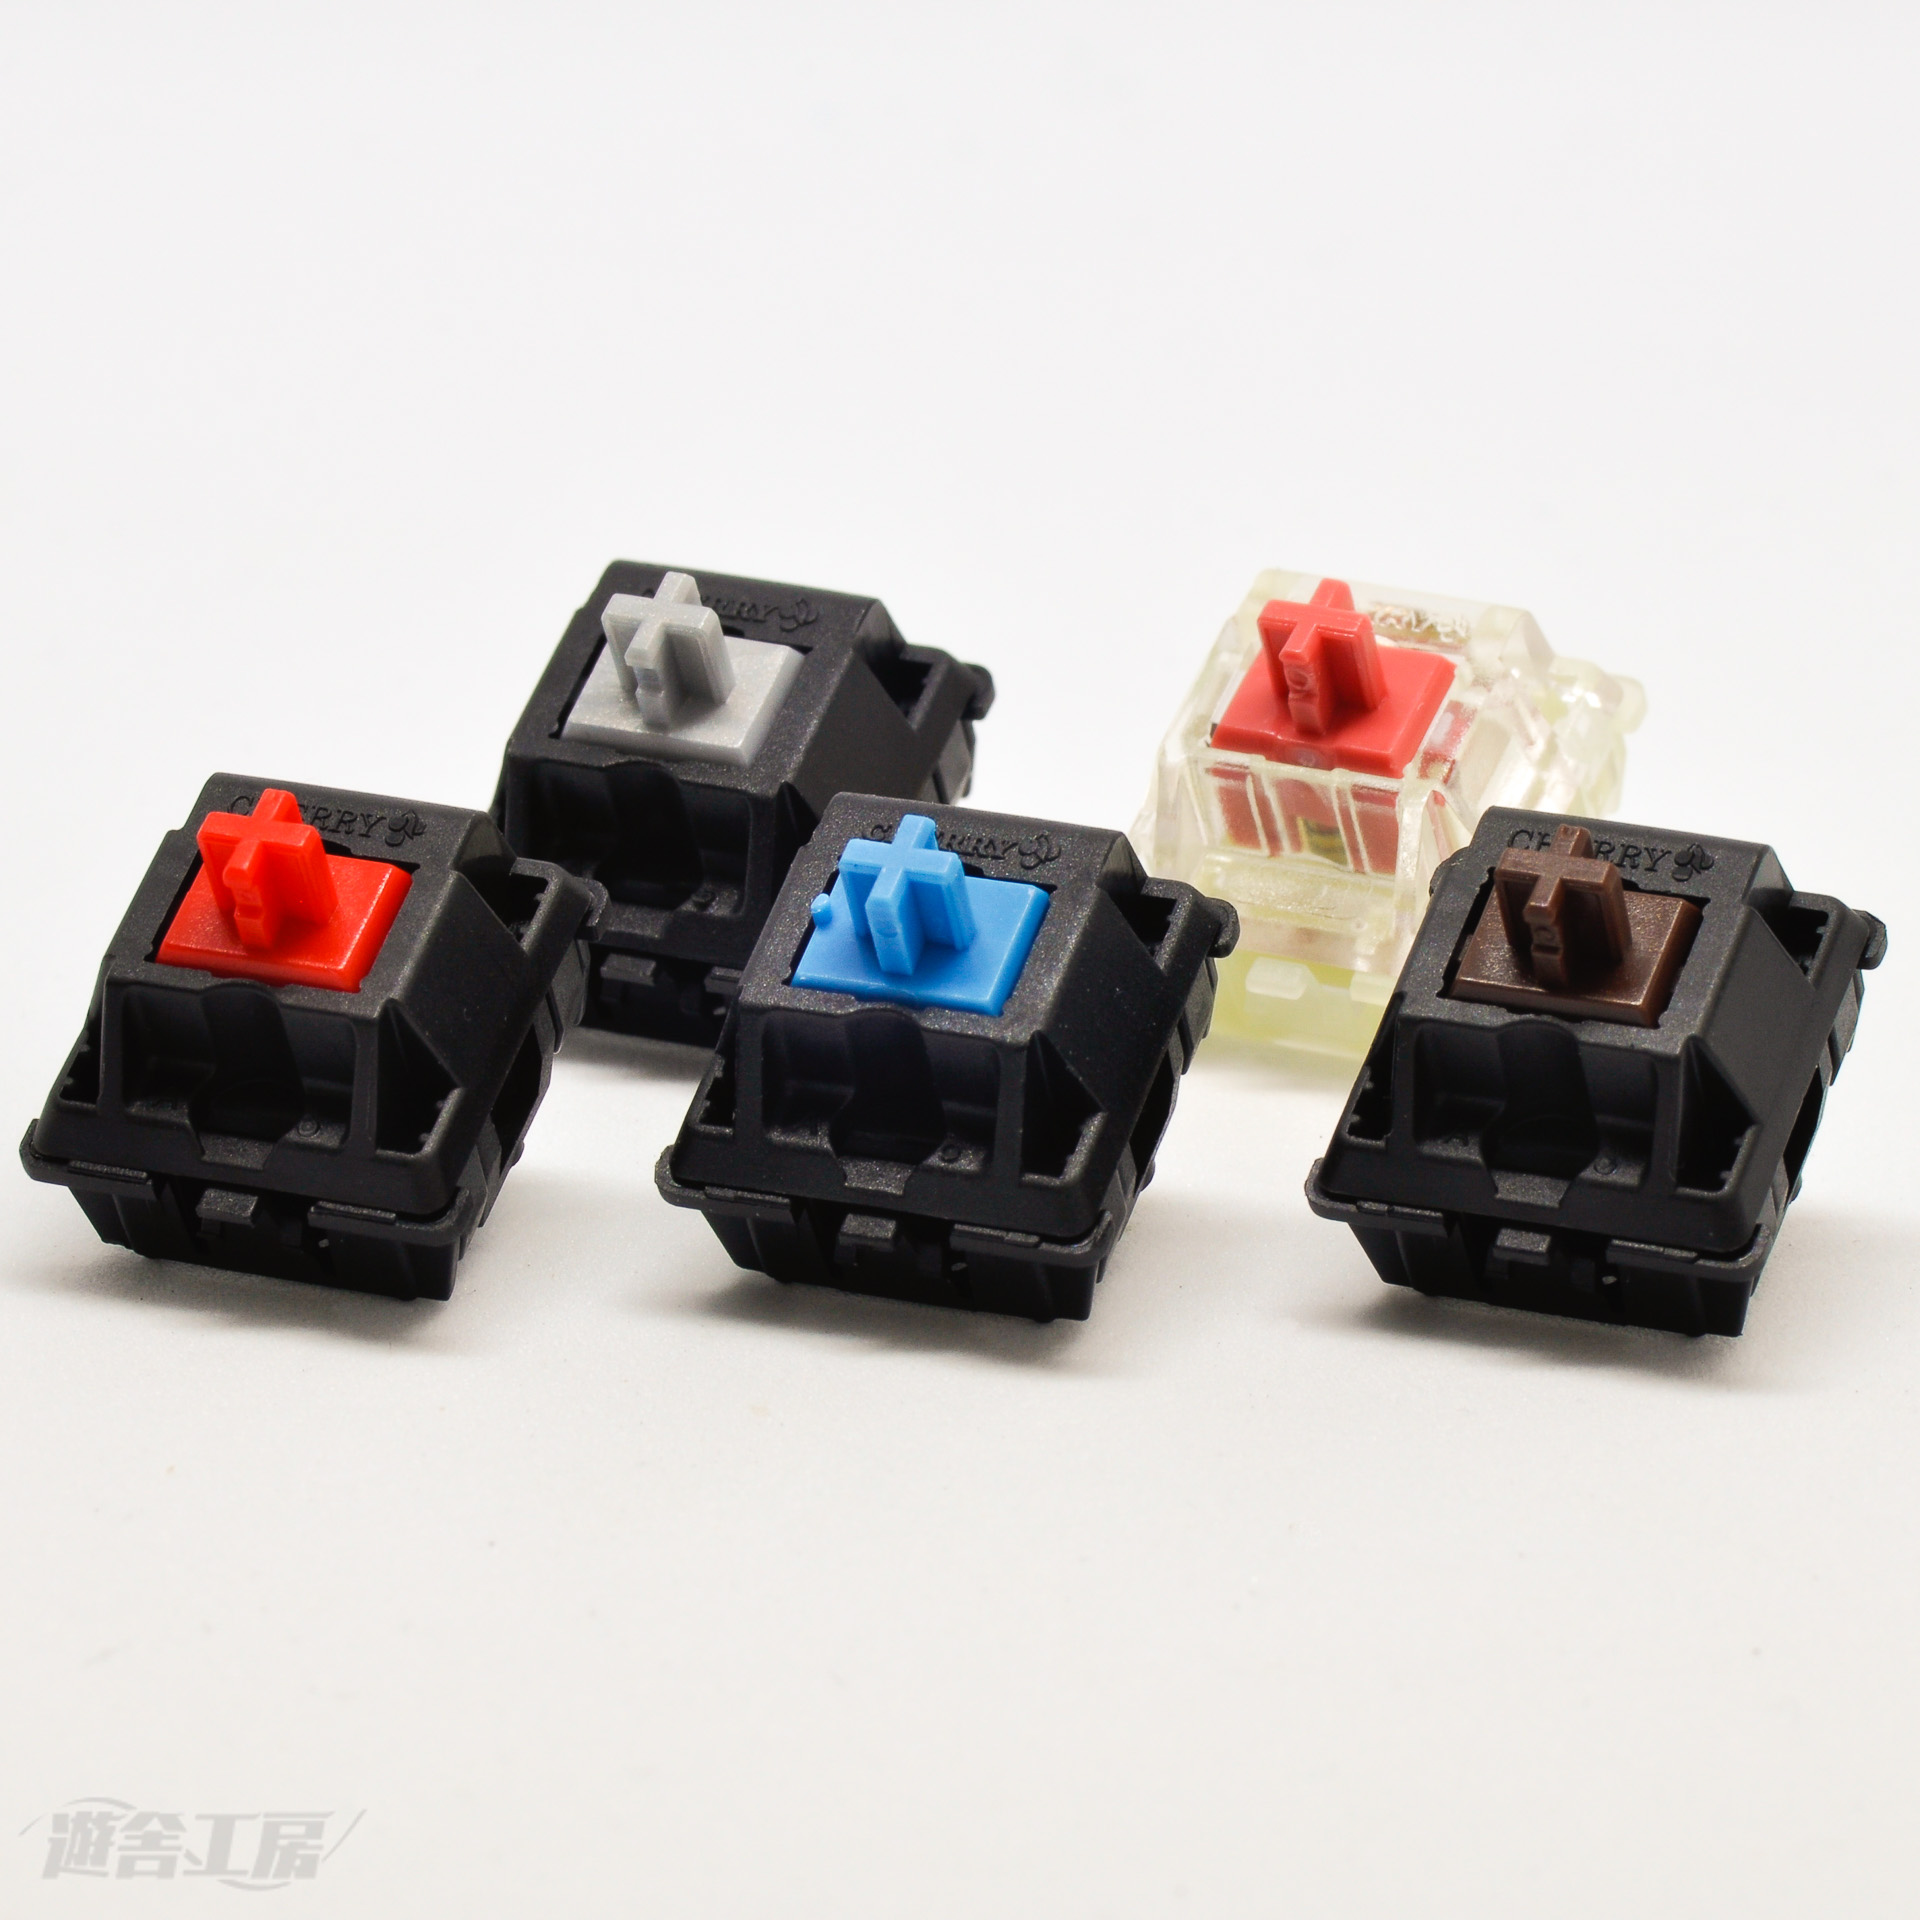
\includegraphics[keepaspectratio,height=3cm]{./img/Cherry_MX-1.jpg}
  \hspace*{1zw}
  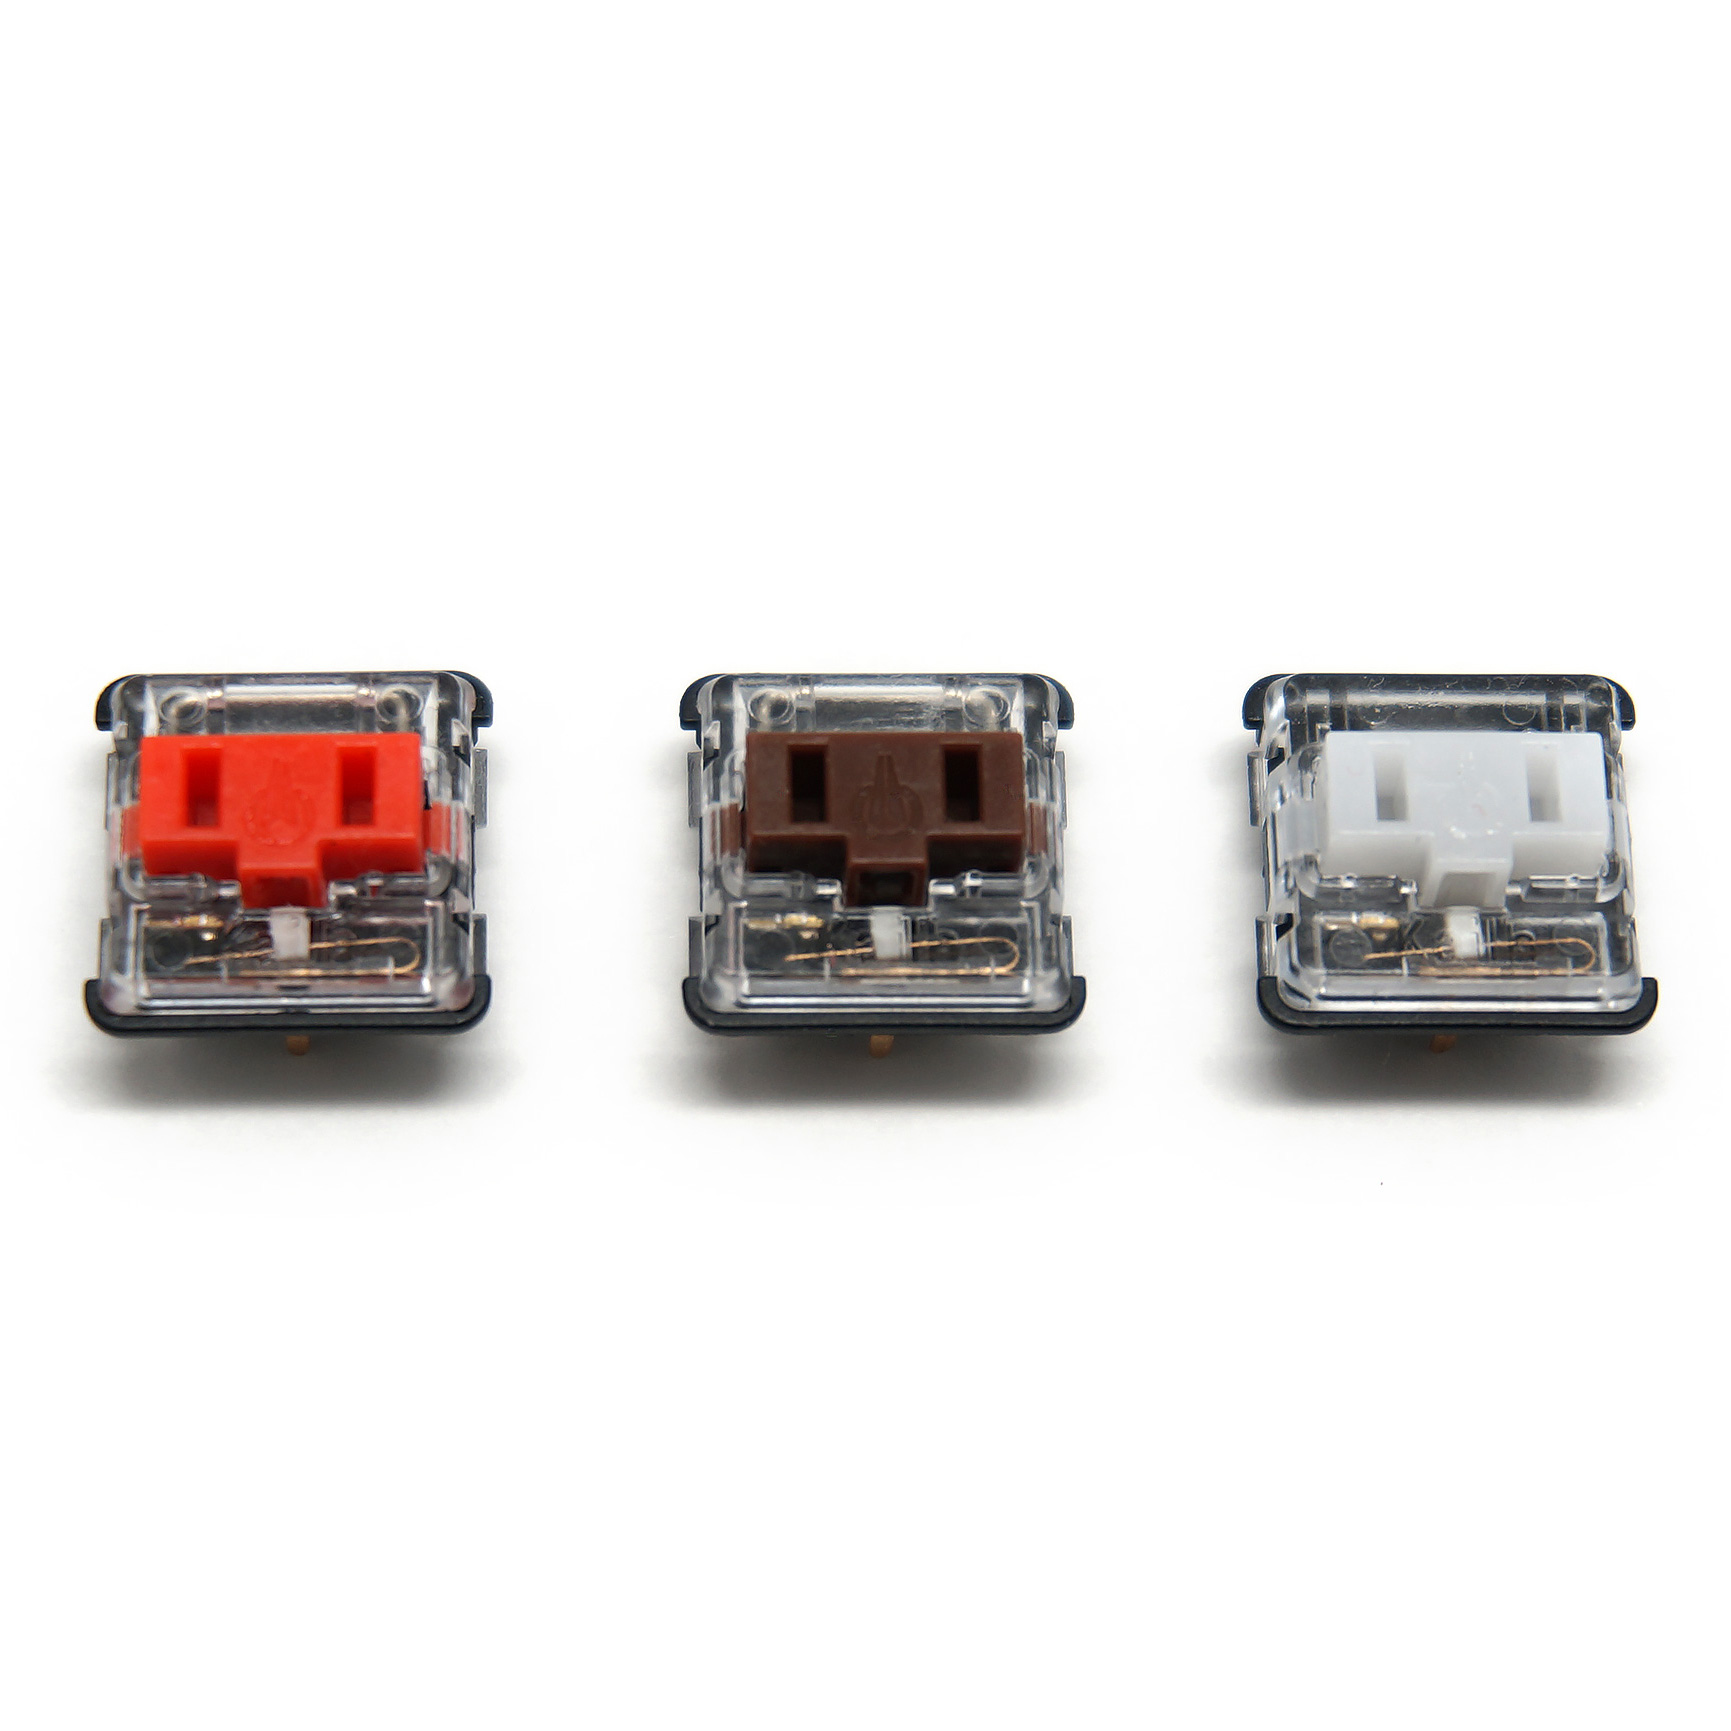
\includegraphics[keepaspectratio,height=3cm]{./img/YKB0003S.jpg}
 \end{center}
 \vspace{-1zw}
 \begin{flushright}
  \footnotesize
  引用元: \url{https://yushakobo.jp/shop/cherry-mx/}, \url{https://yushakobo.jp/shop/pg1350/}
 \end{flushright}
\end{frame}

\begin{frame}[fragile,t]{キースイッチ(2/3)}
 \vspace*{-1zw}
 \begin{center}
  \footnotesize
  \begin{tabular}[tb]{c|cccc}
   軸       & クリック感 & 音       & 重さ   & 深さ \\ \hline
   ピンク軸 & なし       & しずか   & かるめ\\
   赤軸     & なし       & ふつう   & かるめ\\
   茶軸     & あり       & ふつう   & ふつう\\
   黒軸     & なし       & ふつう   & おもめ \\
   青軸     & あり       & カチカチ & おもめ \\
   銀軸     &            &          &        & 浅め
  \end{tabular}
 \end{center}
 \begin{flushright}
  {\footnotesize 参考: \url{https://www.diatec.co.jp/products/CHERRY/}}
 \end{flushright}
 \begin{center}
  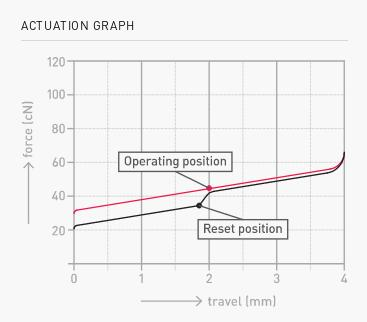
\includegraphics[keepaspectratio,width=3.3cm]{./img/actuation-red.jpg}
  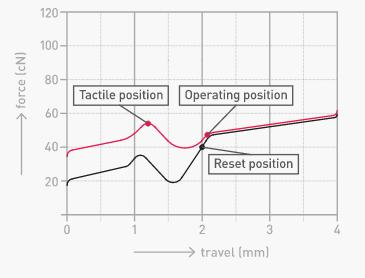
\includegraphics[keepaspectratio,width=3.3cm]{./img/actuation-brown.jpg}
  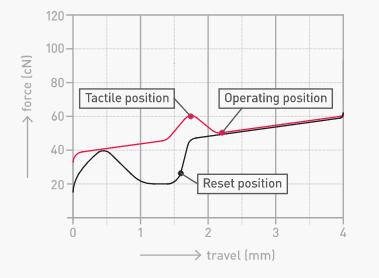
\includegraphics[keepaspectratio,width=3.3cm]{./img/actuation-blue.jpg}
 \end{center}
 \begin{flushright}
  {\footnotesize 引用: \url{https://www.cherrymx.de/en/mx-original/mx-red.html}}
\end{flushright}
\end{frame}

\begin{frame}[fragile,t]{キースイッチ(3/3)}
 \begin{itemize}
  \item 既製品でも軸は選べる
       \begin{itemize}
	\item \textbf{自作だと配置は自由自在}
	\item 小指周りは軽めのスイッチを配置したり
	\item enter keyだけカチカチさせたり
	\item \href{https://yushakobo.jp/shop/a01ps/}{ソケット}を付けておいて後で変更できるようにしたり
       \end{itemize}
 \end{itemize}
 \begin{center}
 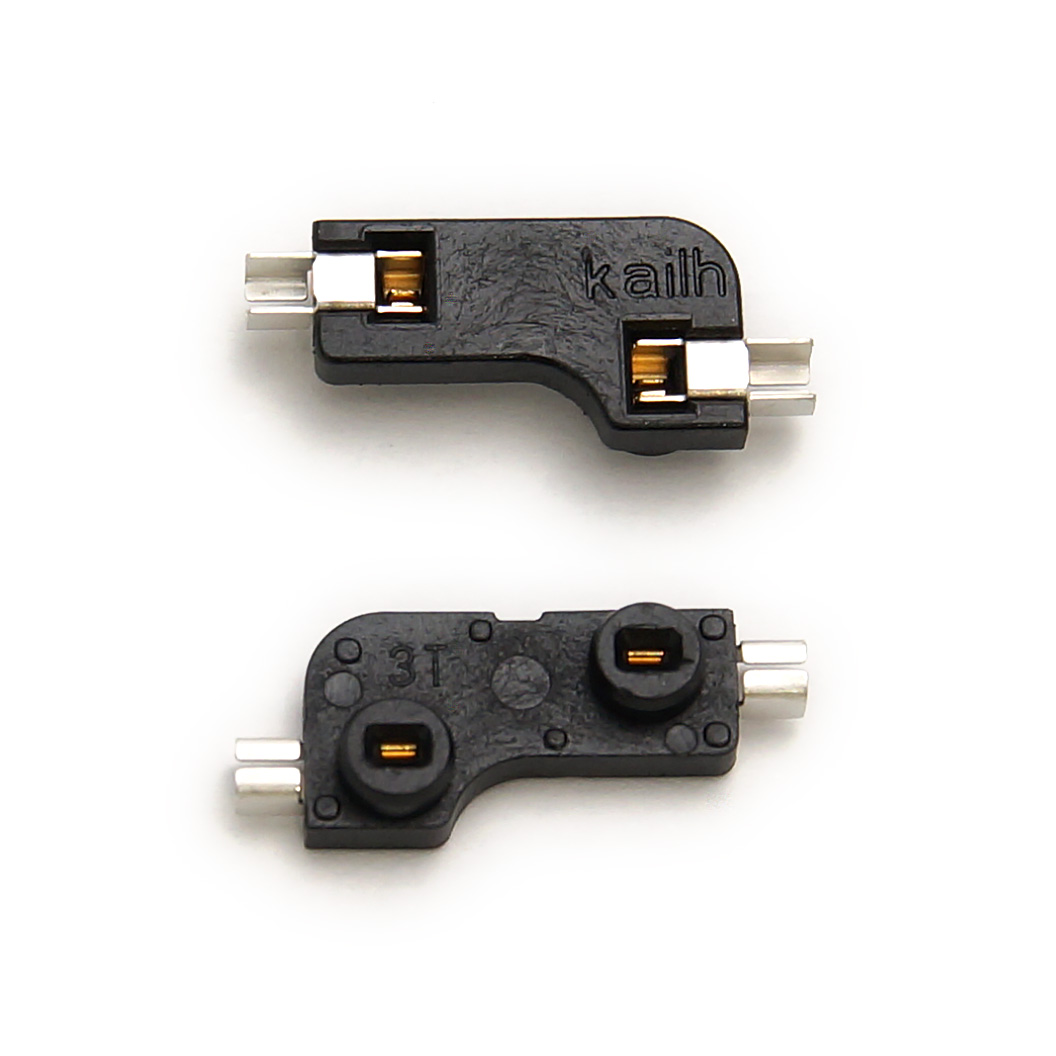
\includegraphics[keepaspectratio,height=2cm]{./img/key-socket.jpg}
 \end{center}
 \begin{flushright}
  \footnotesize 引用元: \url{https://yushakobo.jp/shop/a01ps/}
 \end{flushright}
\end{frame}

\begin{frame}[fragile,t]{マイコン}
 \begin{itemize}
  \item \href{https://www.sparkfun.com/products/12640}{Sparkfun社が出している} Arduino互換ボード
	\begin{itemize}
	 \item Atmel AVR
	 \item とてもコンパクトだけどピン数は結構ある
	 \item ArduinoのIDEが使える
	 \item 定価は結構おたかめ…… \$19.95
	\end{itemize}
  \item Promicroの互換品を使うのが現在の主流
	\begin{itemize}
	 \item おやすい (クローン品だと500円とかで手に入る)
	 \item 情報が多いく、キーボードFW用の環境がある(後述)
	\end{itemize}
 \end{itemize}
\begin{center}
 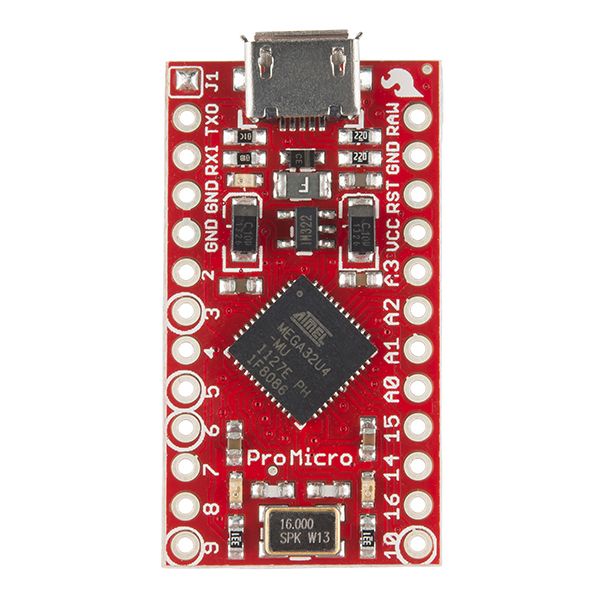
\includegraphics[keepaspectratio,height=3cm]{./img/promicro_01.jpg}
 \hspace*{1zw}
 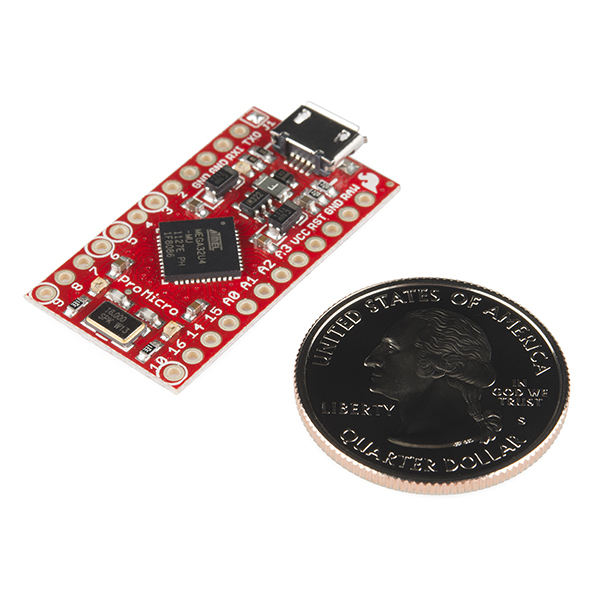
\includegraphics[keepaspectratio,height=3cm]{./img/promicro_02.jpg}
 \hspace*{1zw}
 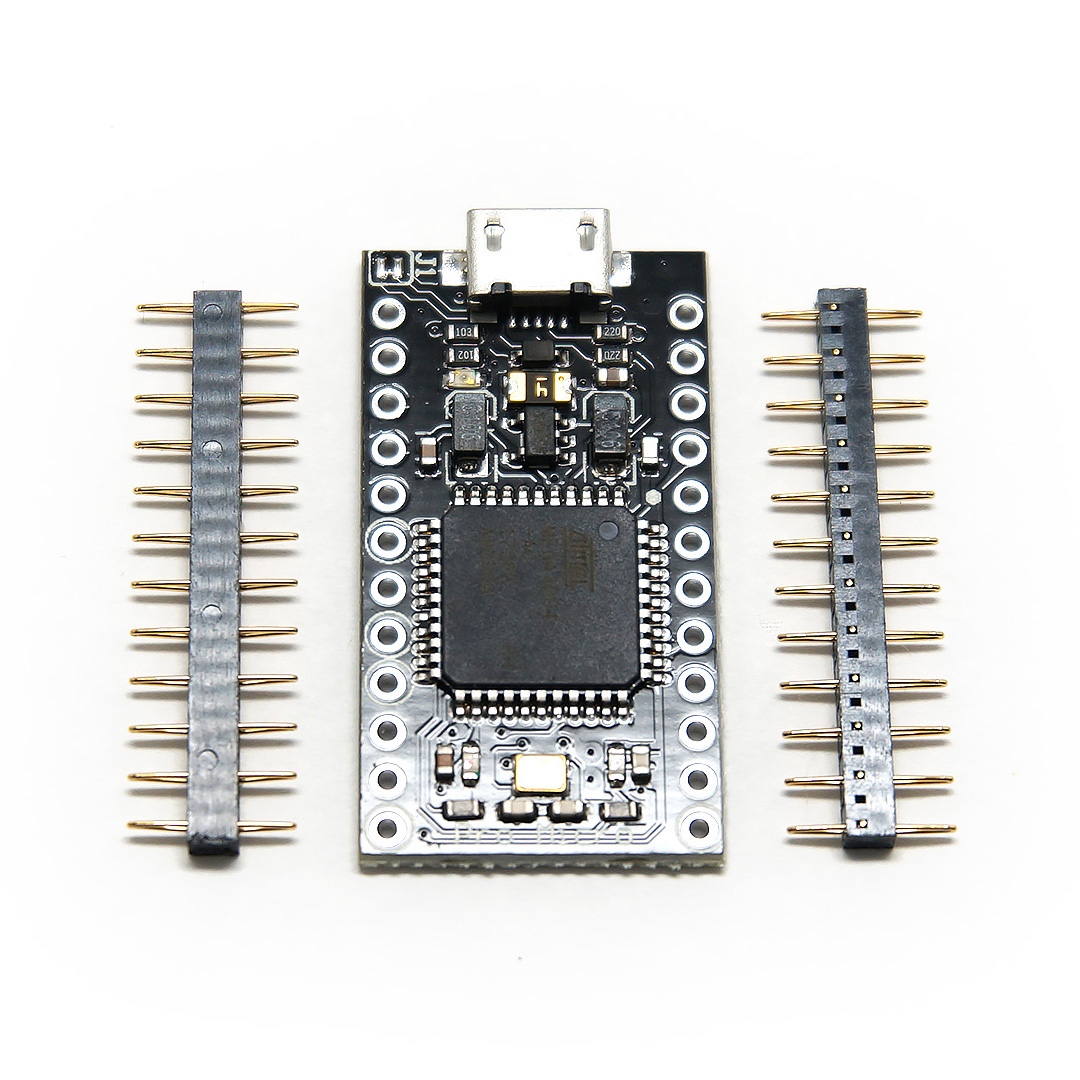
\includegraphics[keepaspectratio,height=3cm]{./img/promicro_compat.jpg}
 \vspace*{-1zw}
\end{center}
\begin{flushright}
 {\footnotesize 引用: \url{https://www.sparkfun.com/products/12640}\\[-.5zw]
 \url{https://yushakobo.jp/shop/promicro-spring-pinheader/}}
\end{flushright}
\end{frame}

\begin{frame}[fragile,t]{キーマトリックス回路}
 \begin{itemize}
  \item さすがにキーボード全てのキーをカバーするほどのピン数はない
  \item キーマトリックス回路をつくってスキャンする
	\begin{itemize}
	 \item 例) 8ピンで16キーを使う場合
	       \begin{itemize}
		\item col0, col1, col2, col3と順次Hiに
		\item 対応するrow0, row1, row2, row3の入力を見る
		\item ダイオードが入ってないと誤判定する
	       \end{itemize}
	\end{itemize}
 \end{itemize}
 \begin{center}
  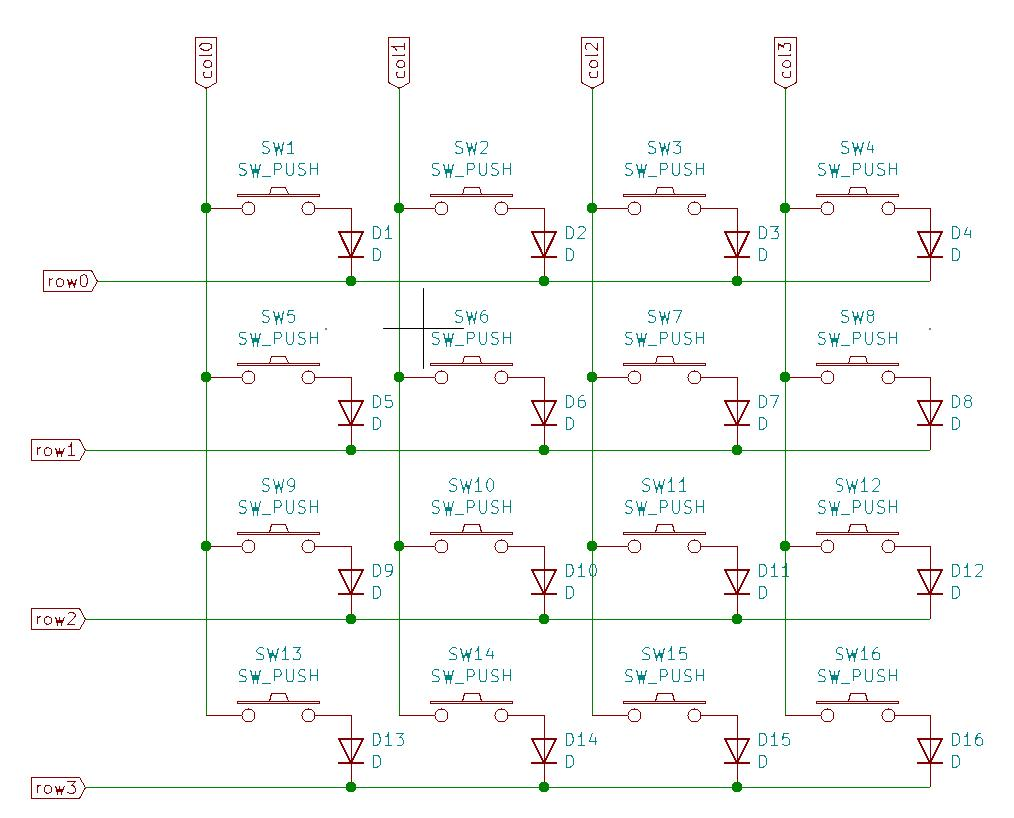
\includegraphics[keepaspectratio,height=4cm]{./img/key-matrix.jpg}
 \end{center}
\end{frame}

\begin{frame}[fragile,t]{分割型キーボード}
 \begin{itemize}
  \item 分割型のキーボードの一般的な構成
	\begin{itemize}
	 \item 左右両方の基板にマイコンを載せる
	       \begin{itemize}
		\item ただし、USBを接続するのは片方だけ
		\item 基板の間を3/4線のシリアル通信させる
	       \end{itemize}
	 \item 通信には3.5mmプラグのケーブル(オーディオでよく使うアレ)を使うのが現在の主流
	       \begin{itemize}
		\item TRS(3極: モノラルケーブル)
		\item TRRS(4極: ステレオケーブル)
	       \end{itemize}
	 \item TRSの場合は通信時に送受信を切り替えて実施している
	       \begin{itemize}
		\item VCC/GNDで2極使用するため
		\item かつてはTRRSのケーブルやらジャックが入手しづらかったらしい?
	       \end{itemize}
	 \item 海外のキーボードミートアップではあまりみかけないらしい
	\end{itemize}
 \end{itemize}
\end{frame}

\begin{frame}[fragile,t]{LED / OLED}
 \begin{itemize}
  \item キーボードは格好良くなくてはいけない!!
  \item LED
	\begin{itemize}
	 \item LEDチップをキーの後ろにつけて文字を光らせる
	 \item LEDテープで机を光らせる
	 \item LEDチップのはんだ付けはちょっと難易度高め
	\end{itemize}
  \item OLED
	\begin{itemize}
	 \item I2Cのお安いOLEDをつけるのも流行ってる
	 \item モード状態やキーボードのロゴを表示させるのに利用
	 \item Arduino用のライブラリもあるので結構遊べそう
	\end{itemize}
 \end{itemize}
 \begin{center}
  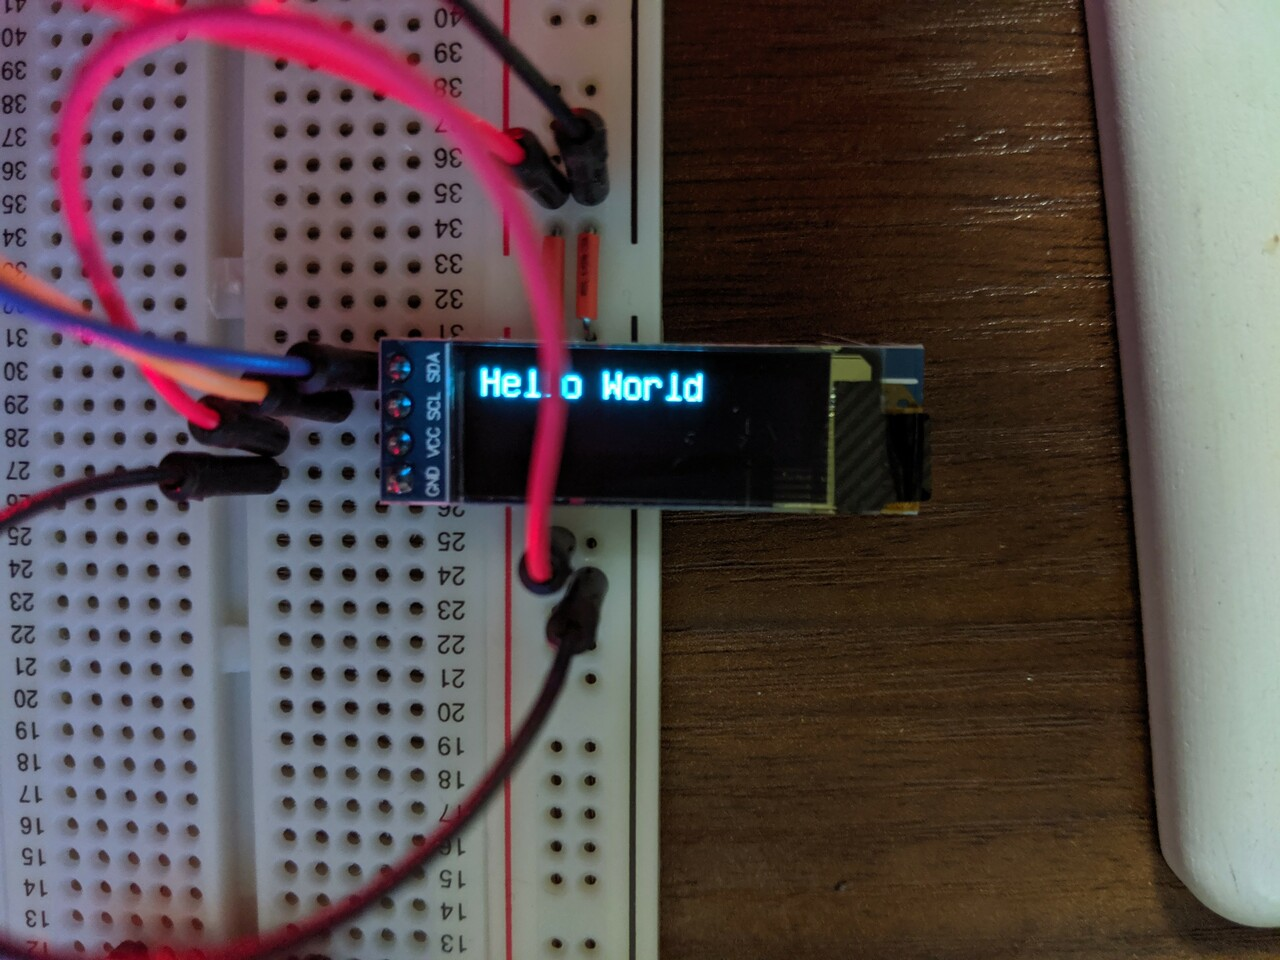
\includegraphics[keepaspectratio,height=2.5cm]{./img/oled-hello-world.jpg}
 \end{center}
\end{frame}

\begin{frame}[fragile,t]{キーボードの組み立てに必要なもの}
 \begin{itemize}
  \item 必須
	\begin{itemize}
	 \item はんだ (素直に鉛入りを使いましょう。換気注意。)
	 \item はんだごて (温調可能なものがベター。LEDチップを付けるならほぼ必須)
	 \item はんだごて台 (汚れ落としは水を使わないやつの方が良い)
	\end{itemize}
  \item 準必須
	\begin{itemize}
	 \item ラジオペンチ
	 \item ニッパー (ダイオードが素子タイプなら必須)
	 \item ピンセット (ダイオードやLEDがチップタイプなら必須)
	\end{itemize}
  \item 推奨
	\begin{itemize}
	 \item テスター
	 \item はんだ吸い取り器 (吸い取り線は難易度高め)
	\end{itemize}
 \end{itemize}
\end{frame}

\begin{frame}[fragile,t]{Mint60組み立て (1/4)}
 \begin{itemize}
  \item 開封!!
 \end{itemize}
 \begin{center}
 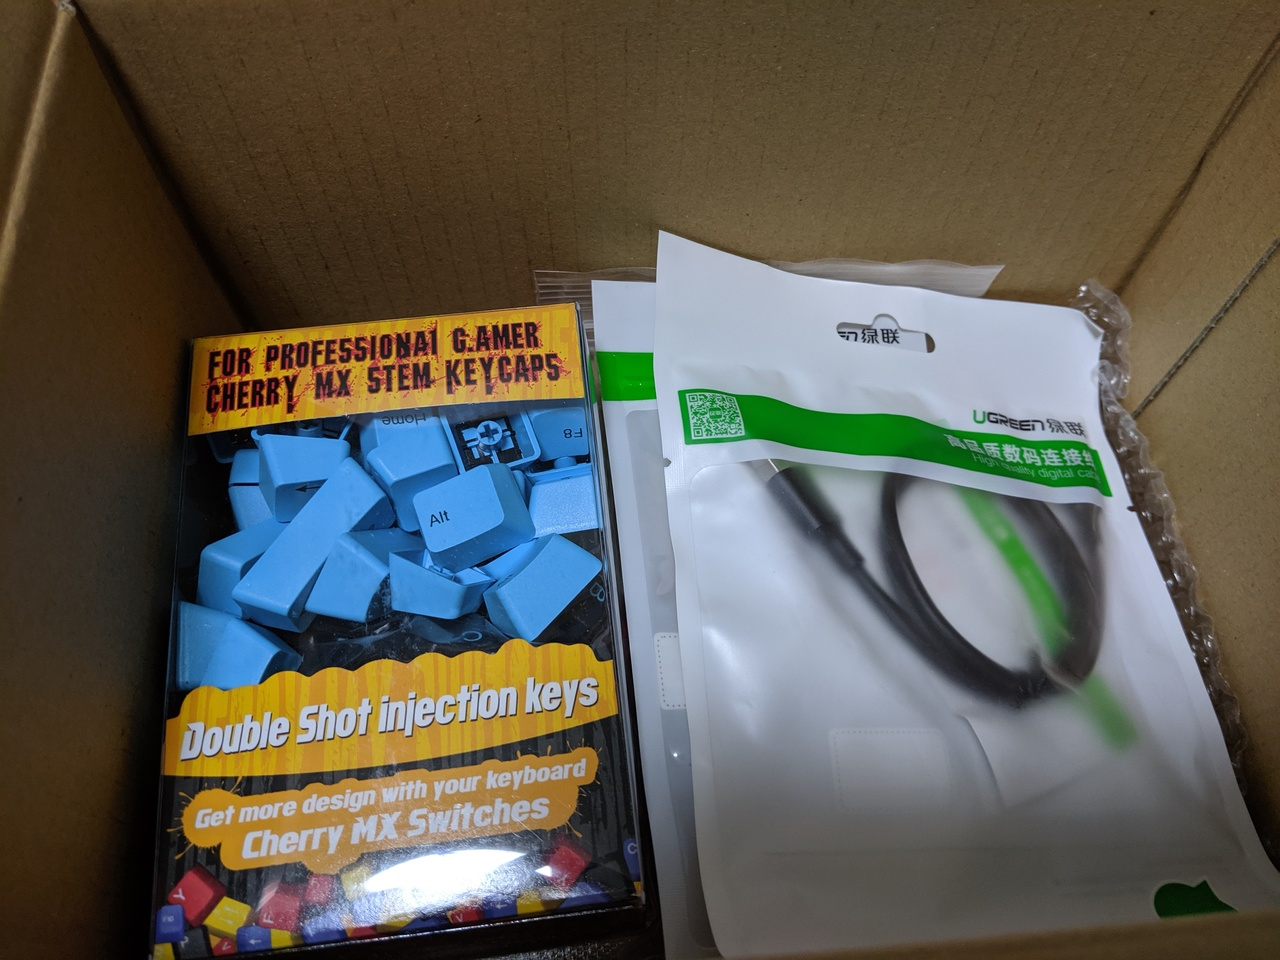
\includegraphics[keepaspectratio,height=3cm]{./img/mint60-unpack-01.jpg} \hspace*{1zw}
 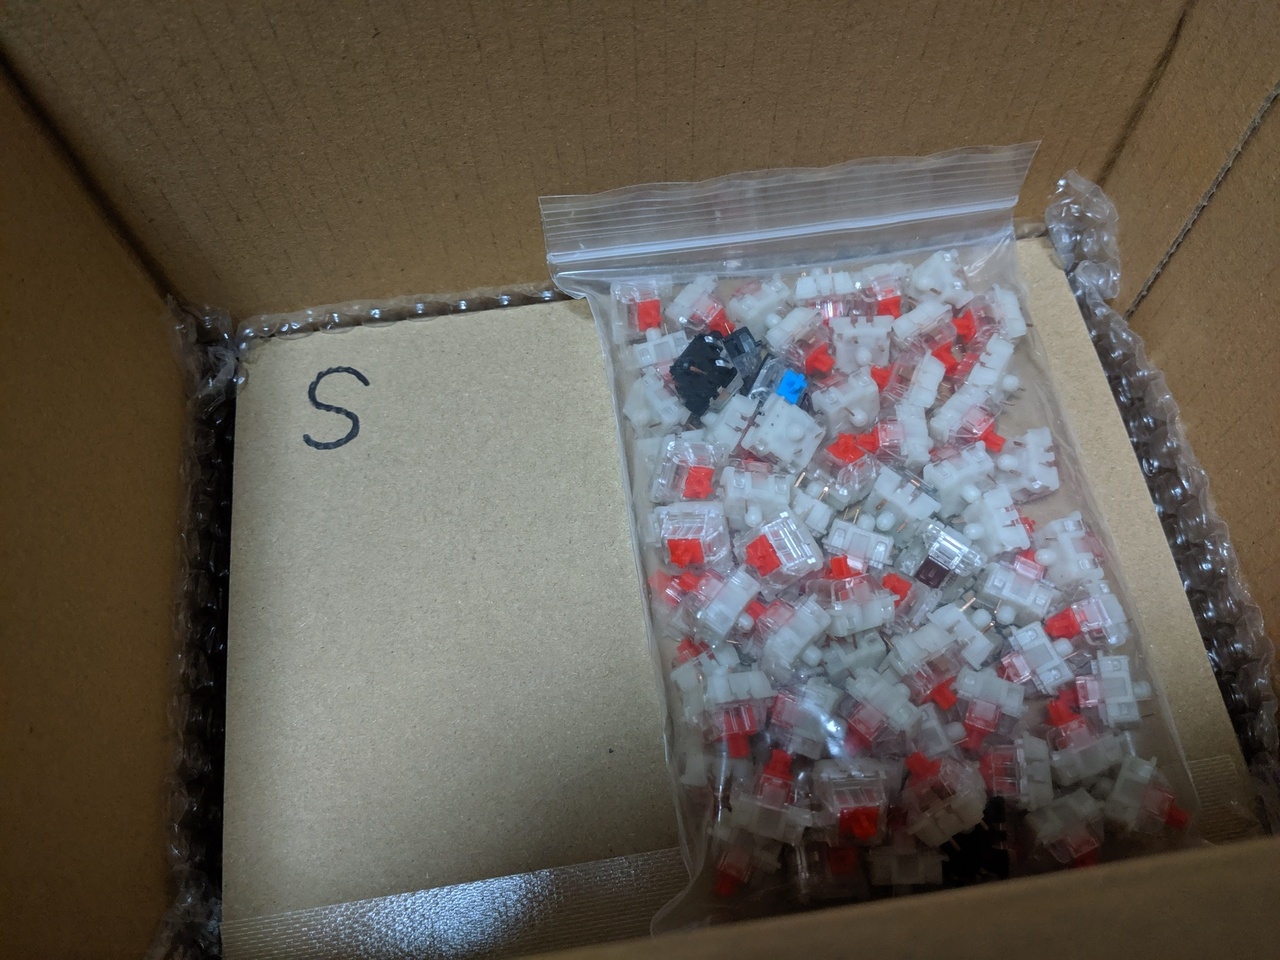
\includegraphics[keepaspectratio,height=3cm]{./img/mint60-unpack-02.jpg} \\
 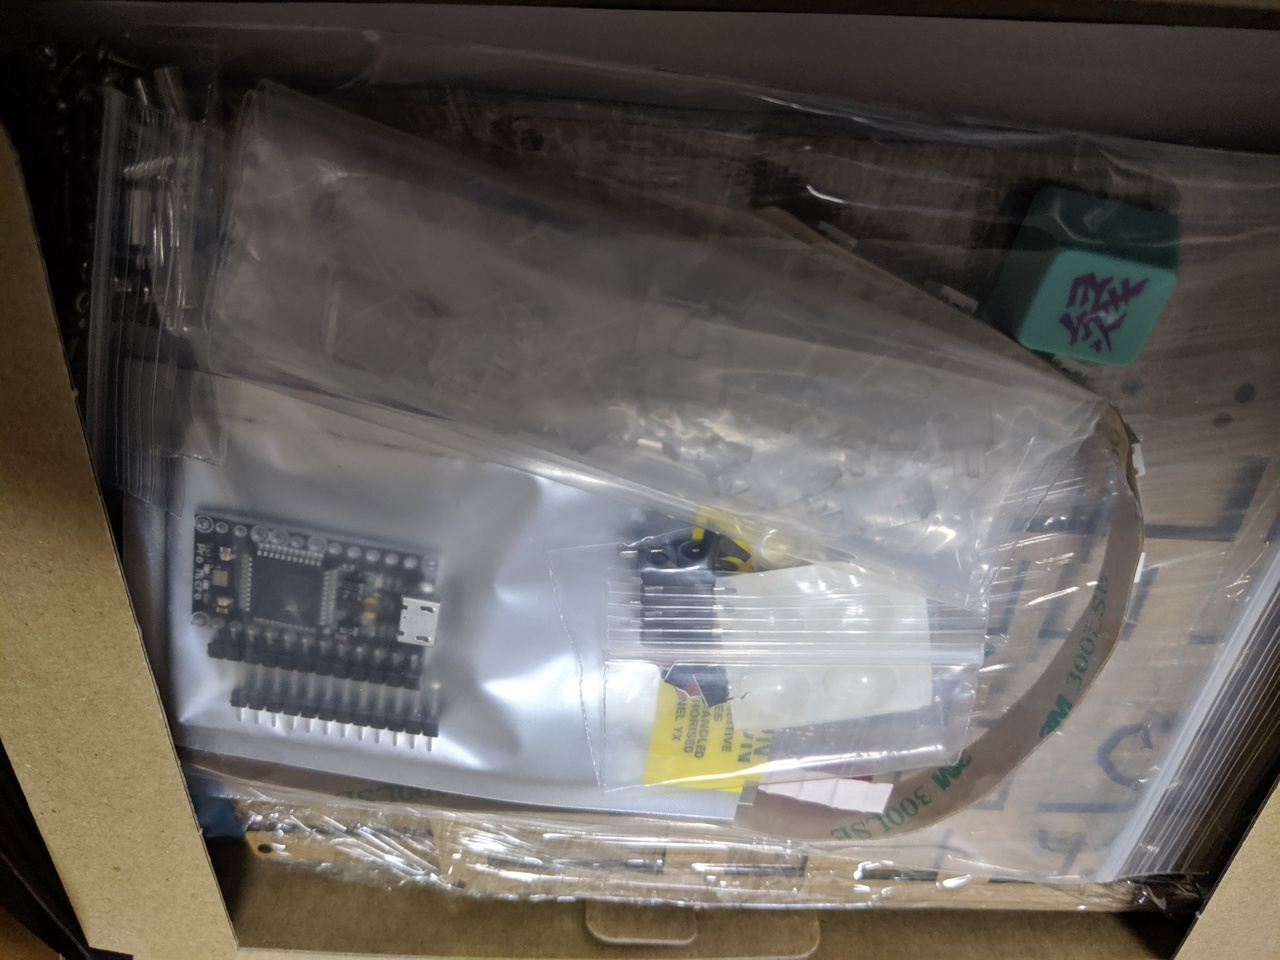
\includegraphics[keepaspectratio,height=3cm]{./img/mint60-unpack-03.jpg}
 \end{center}
\end{frame}

\begin{frame}[fragile,t]{Mint60組み立て (2/4)}
 \begin{itemize}
  \item 組み立てるぜ!!
 \end{itemize}
 \begin{center}
  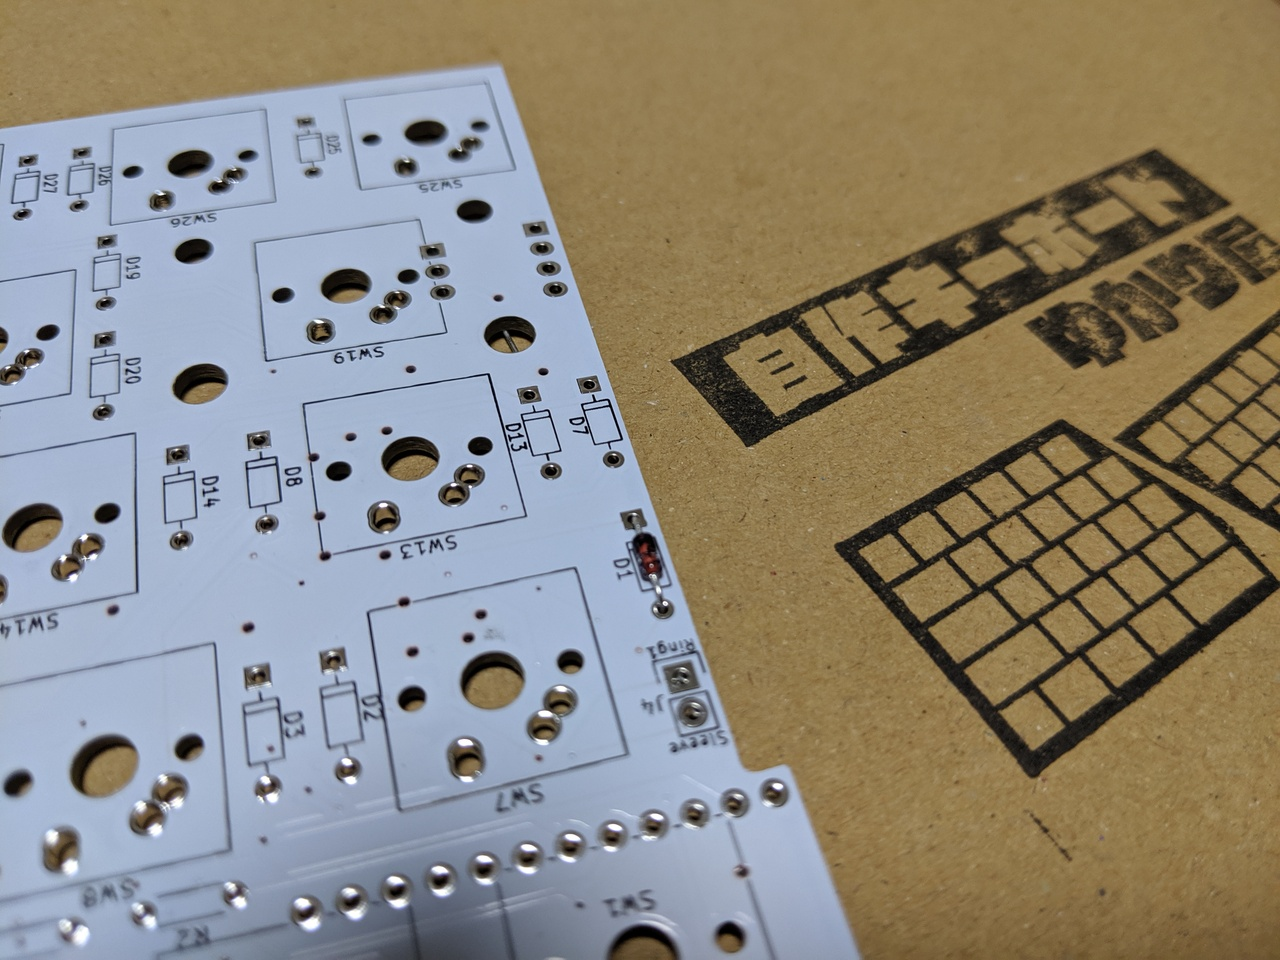
\includegraphics[keepaspectratio,height=3cm]{./img/mint60-build-01.jpg} \hspace*{1zw}
  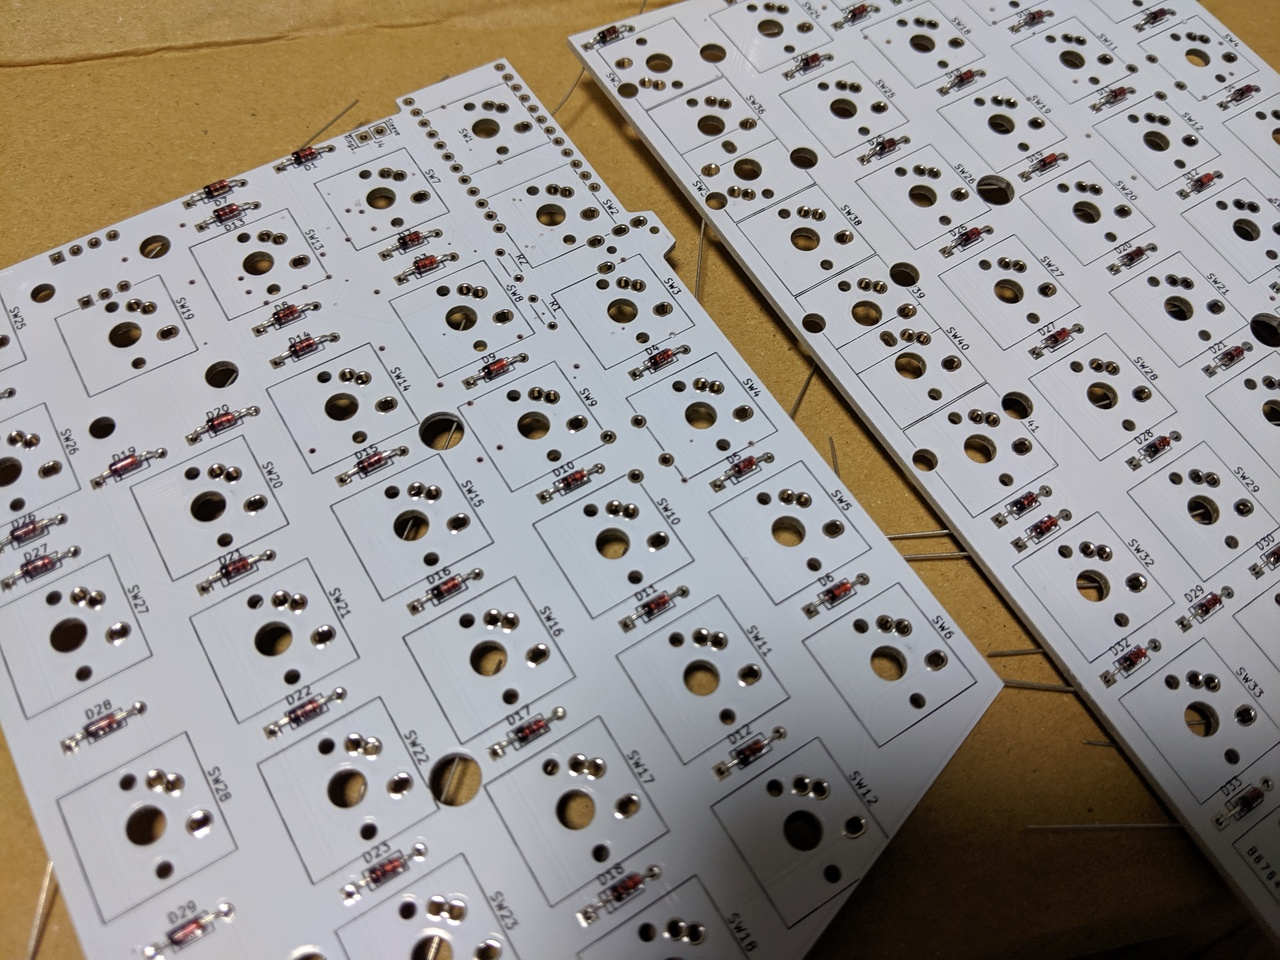
\includegraphics[keepaspectratio,height=3cm]{./img/mint60-build-02.jpg} \\
  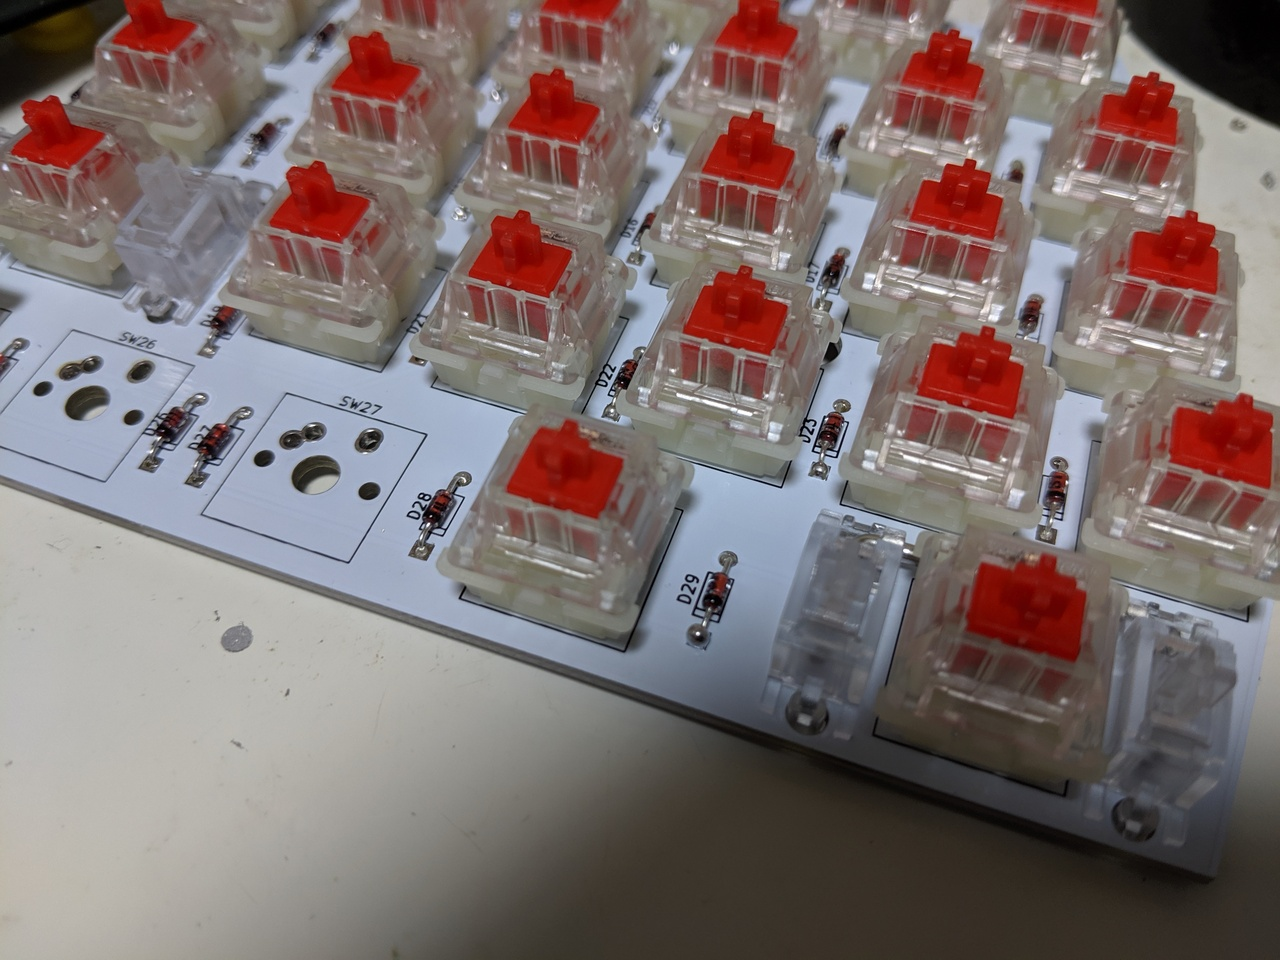
\includegraphics[keepaspectratio,height=3cm]{./img/mint60-build-03.jpg} \hspace*{1zw}
  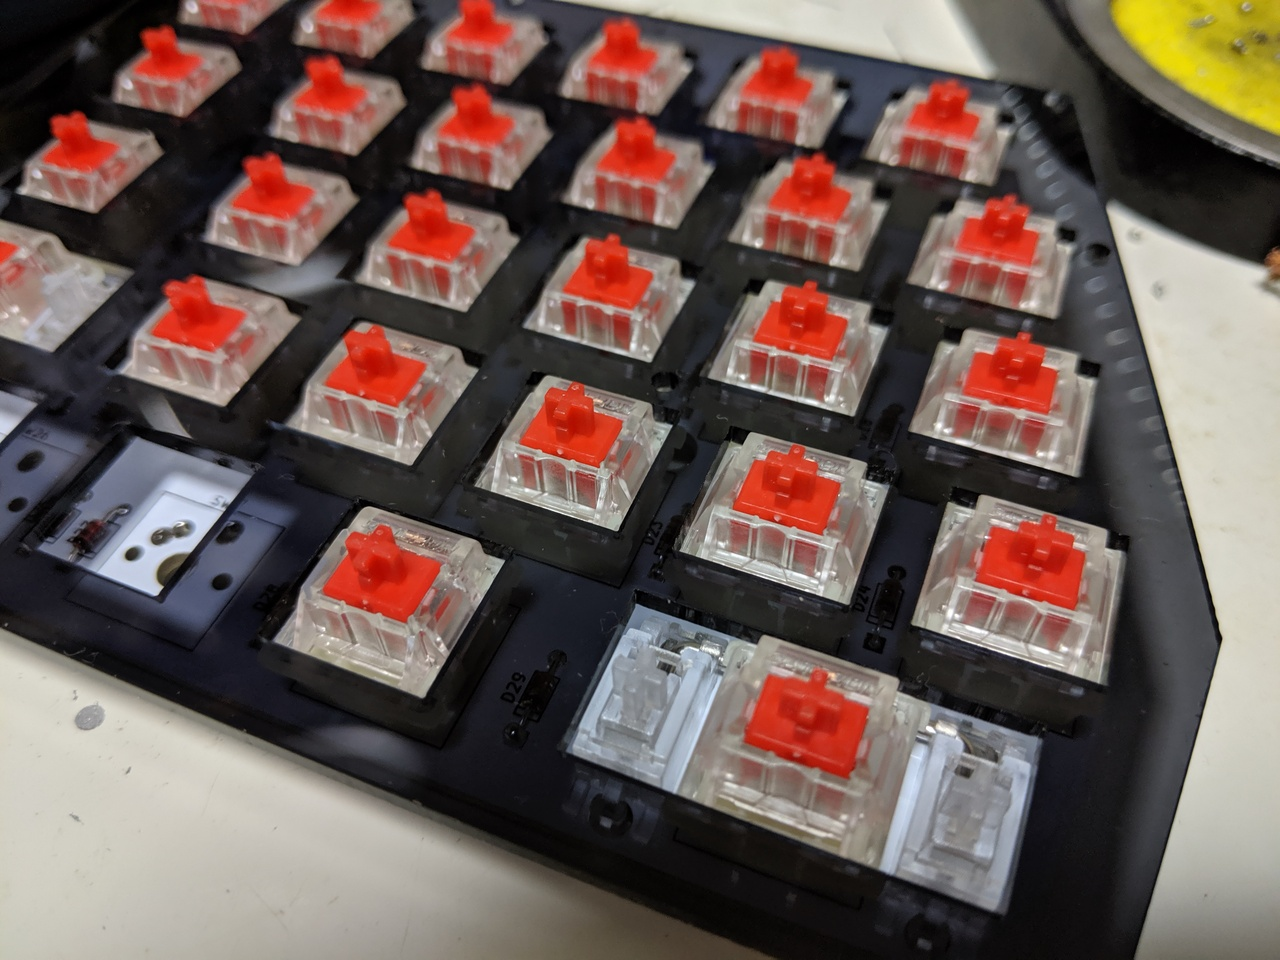
\includegraphics[keepaspectratio,height=3cm]{./img/mint60-build-04.jpg}
 \end{center}
\end{frame}

\begin{frame}[fragile,t]{Mint60組み立て (3/4)}
 \begin{itemize}
 \onslide<2->{\item 実はとんでもなくやらかしています}
 \end{itemize}
 \vspace*{-1zw}
 \begin{center}
  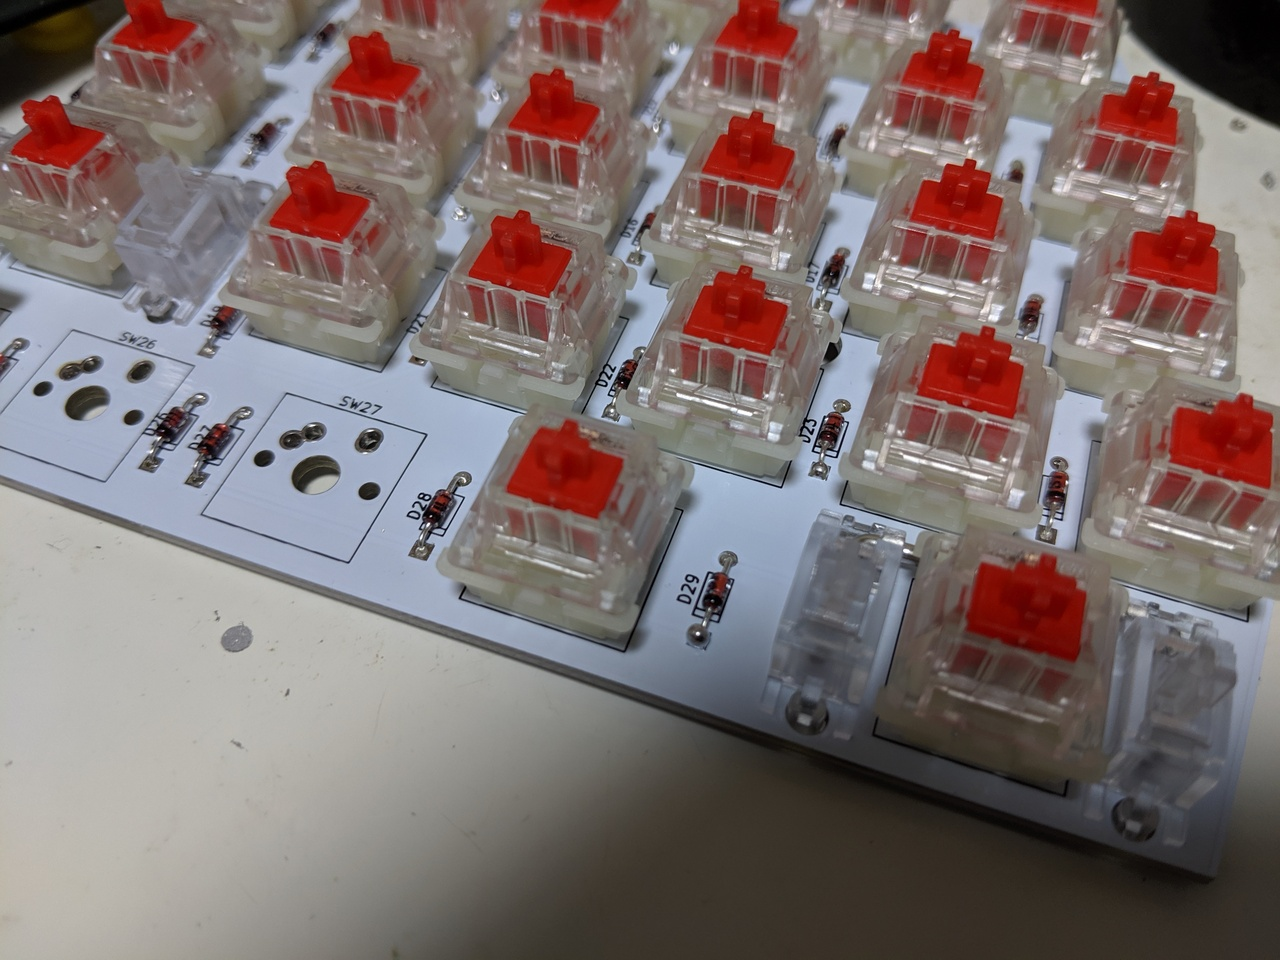
\includegraphics[keepaspectratio,height=4cm]{./img/mint60-build-03.jpg} \hspace*{1zw}
  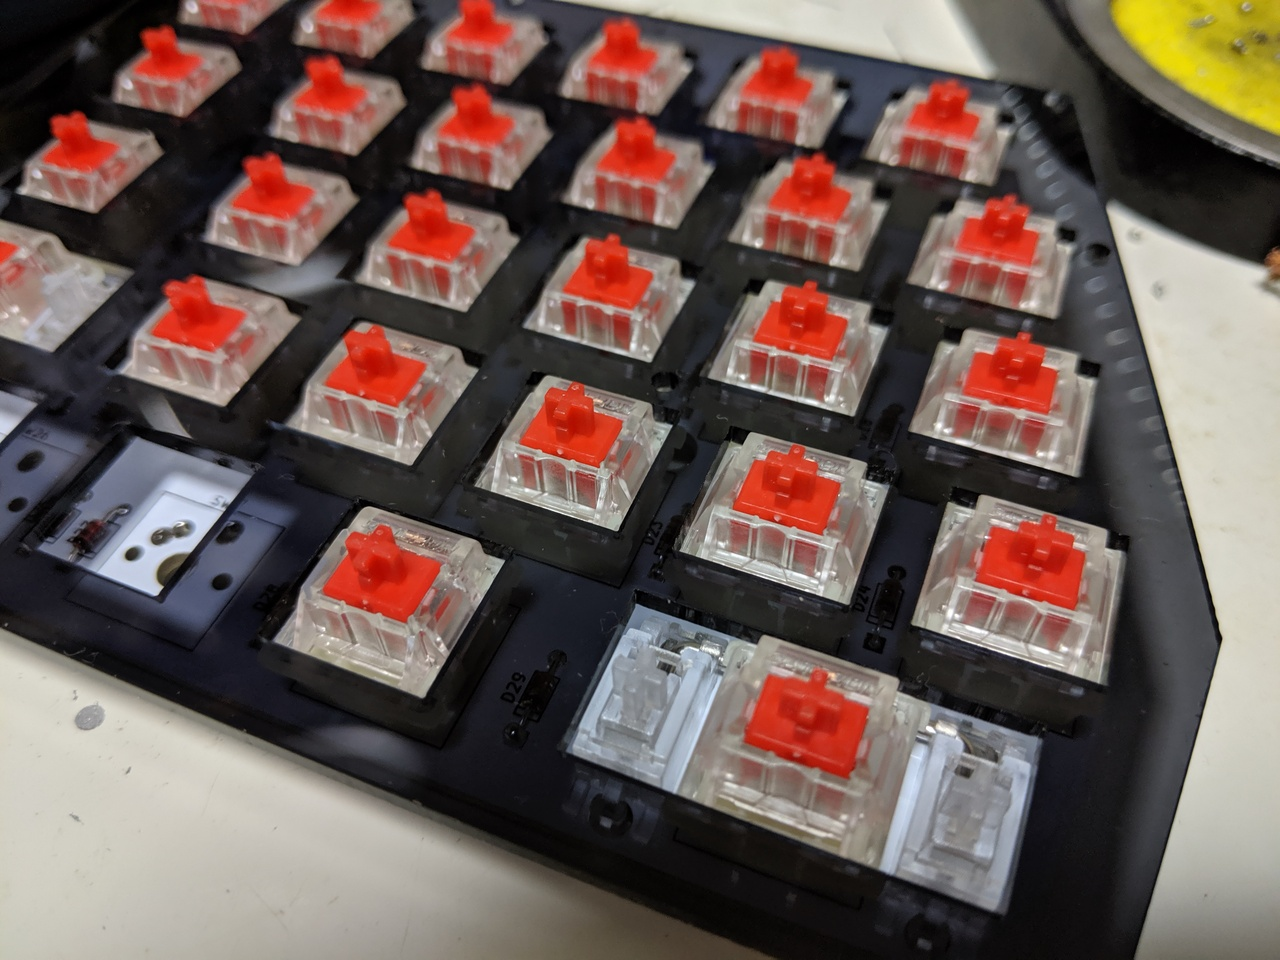
\includegraphics[keepaspectratio,height=4cm]{./img/mint60-build-04.jpg}
 \end{center}
 \vspace*{-1zw}
 \begin{itemize}
 \onslide<3->{\item 正しい手順: 基板→アクリル版→キースイッチ}
 \onslide<4->{\item バカ: 基板→キースイッチ→アクリル版}
		    \begin{itemize}
		     \onslide<5->{\item バカ「キーキャップはまり悪い」「アクリルカバーでうまく挟めない」}
		    \end{itemize}
 \end{itemize}
\end{frame}

\begin{frame}[fragile,t]{Mint60組み立て (4/4)}
 \begin{itemize}
  \item 泣きながらキースイッチを外す
 \end{itemize}
 \begin{center}
  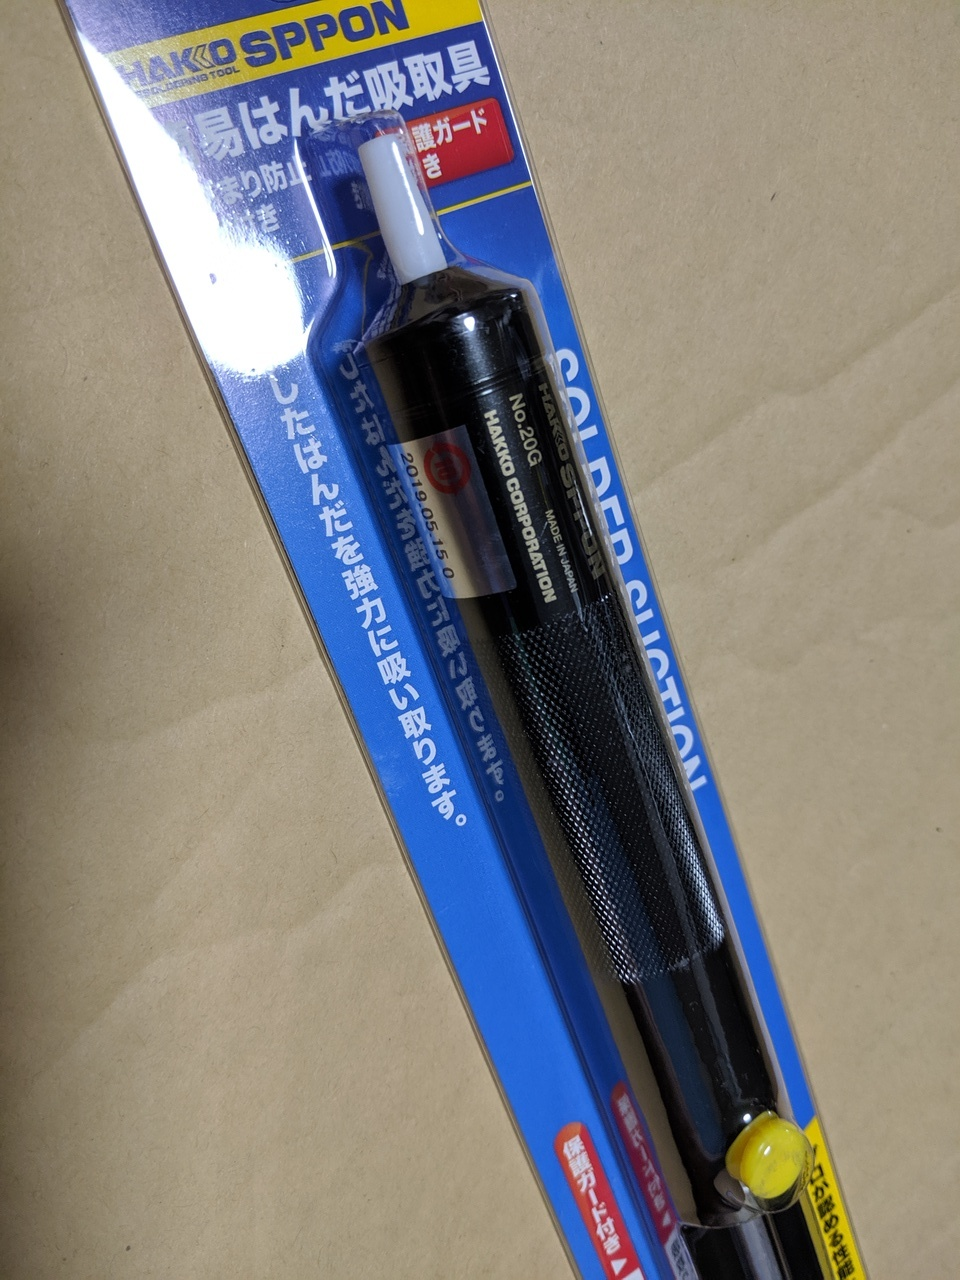
\includegraphics[keepaspectratio,height=4cm]{./img/mint60-build-05.jpg} \hspace*{.3zw}
  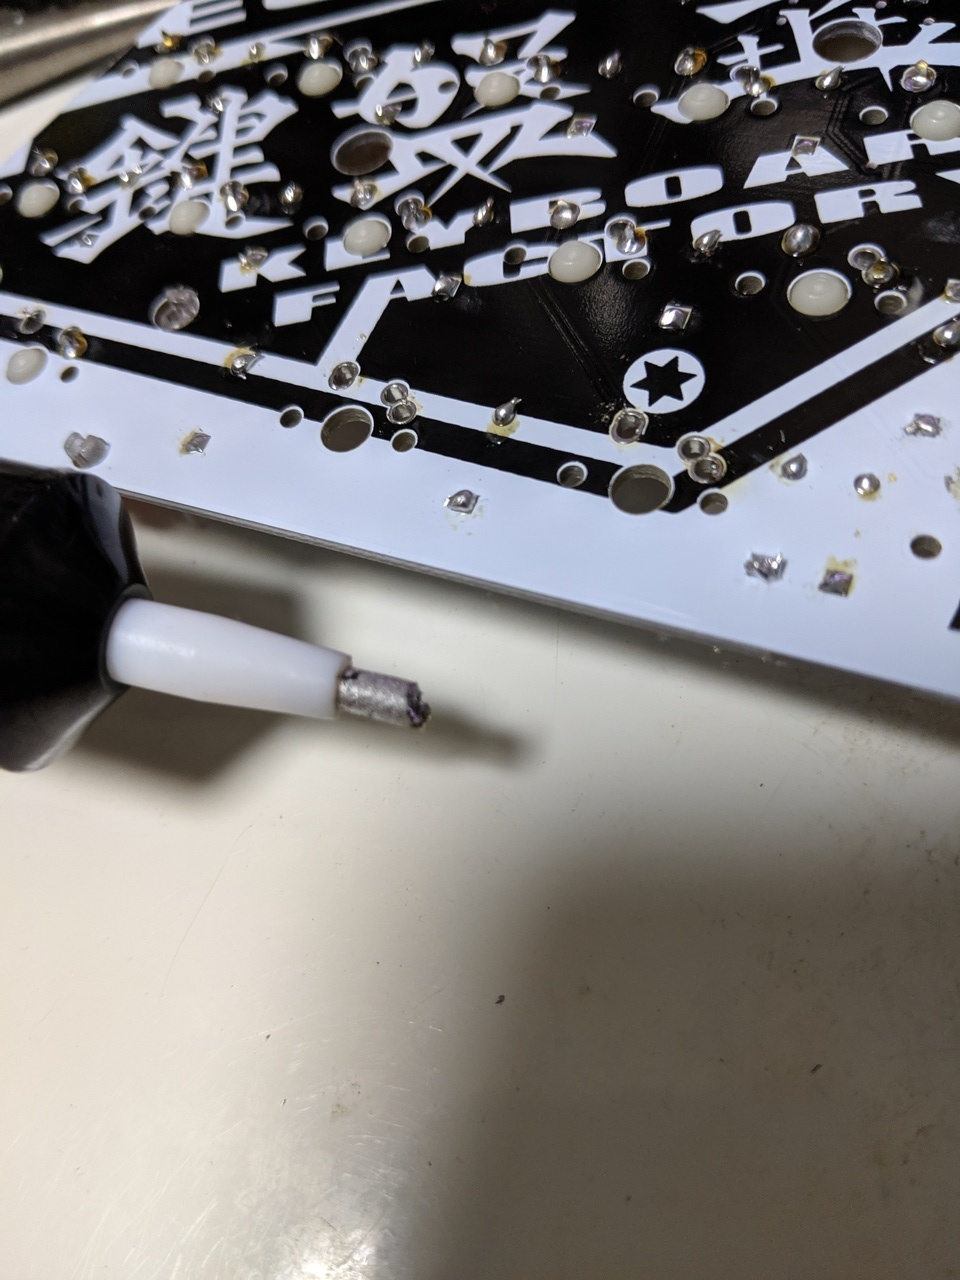
\includegraphics[keepaspectratio,height=4cm]{./img/mint60-build-06.jpg} \hspace*{.3zw}
  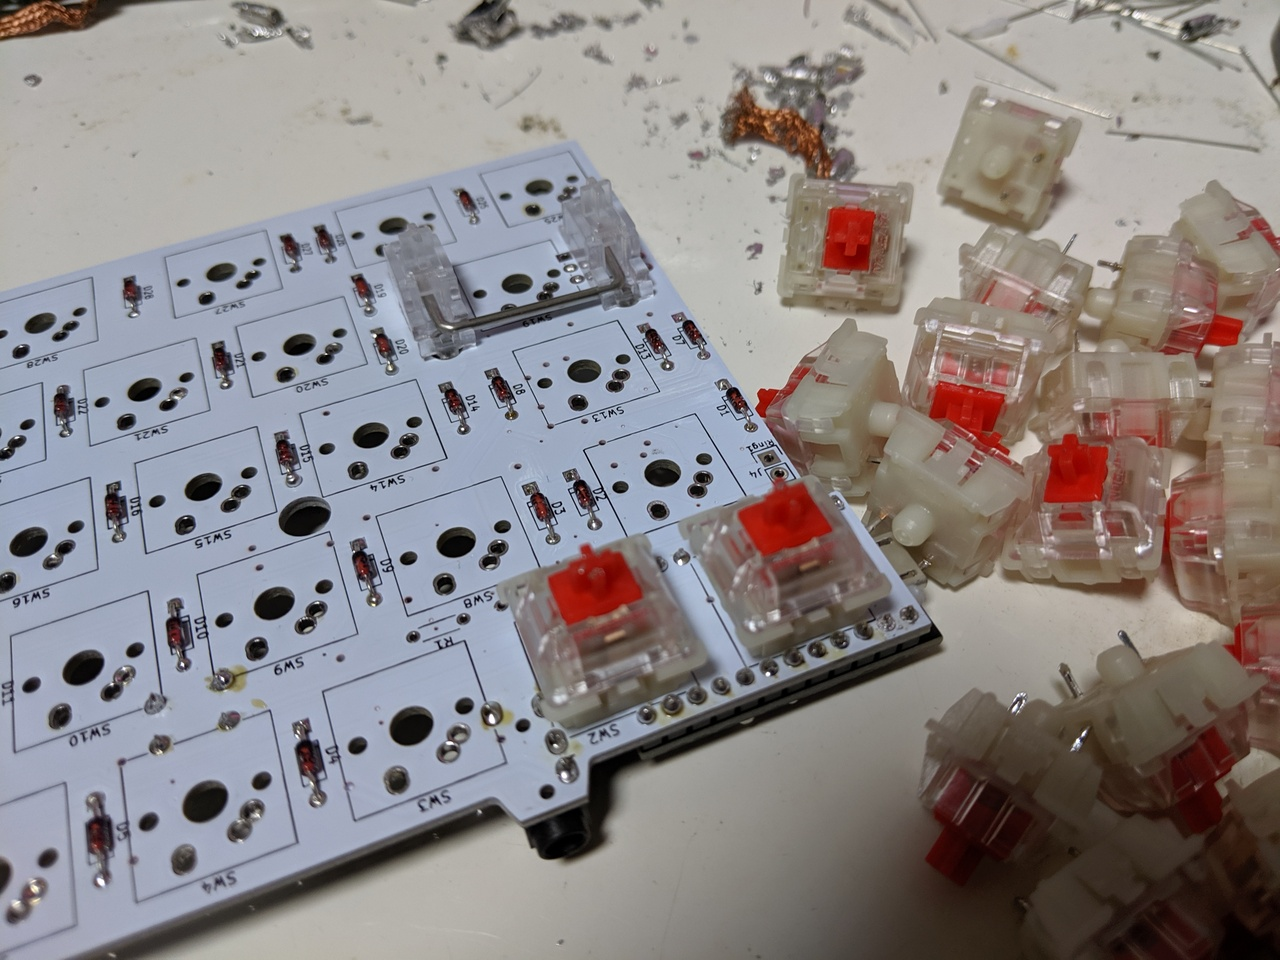
\includegraphics[keepaspectratio,height=4cm]{./img/mint60-build-07.jpg}
 \end{center}
 \begin{itemize}
  \onslide<2->{\item で、なんとか完成するもシリアル通信できず}
  \onslide<3->{\item それぞれにUSBケーブル挿して運用中……}
 \end{itemize}
\end{frame}

\begin{frame}[fragile,t]{Mint60 使い心地}
 \begin{itemize}
  \item 基本ホームポジション遵守派なので違和感少なめ
	\begin{itemize}
	 \item 自分が6を右手でも左手でも打ってる事に気付いた(Mint60では右手のみ)
	 \item スペースキーは基本右手だが、カーソルキーに手があると左手で押していた
	\end{itemize}
  \item 肩凝り緩和を期待していたが、むしろ腰痛に効いた!!
 \end{itemize}
\end{frame}

\begin{frame}[fragile,t]{ファームウェアのカスタマイズ (1/4)}
 \begin{itemize}
  \item 主な自作キーボードキットは \href{https://qmk.fm/}{QMK Firmware} を利用している
	\begin{itemize}
	 \item Atmel AVRマイコンやARMのキーボード用ファーム
	 \item 単純な設定ファイルを書くだけで新規FWを作れる
	 \item Mint60やHelixはアップストリームにマージ済み
	\end{itemize}
  \item Debianで使うには
 \end{itemize}
 \begin{commandline}
% sudo apt install gcc unzip wget zip gcc-avr binutils-avr avr-libc \
dfu-programmer dfu-util gcc-arm-none-eabi binutils-arm-none-eabi \
libnewlib-arm-none-eabi
 \end{commandline}
 \pause
 \begin{itemize}
  \item その後以下のようにビルドできる
	\begin{itemize}
	 \item (機種名):(キーマップ名)
	\end{itemize}
 \end{itemize}
 \begin{commandline}
% make helix:default
% make mint60:default
 \end{commandline}
\end{frame}

\begin{frame}[fragile,t]{ファームウェアのカスタマイズ (2/4)}
 \begin{itemize}
  \item キーの入れ替え等は簡単にできる
	\begin{itemize}
	 \item \verb|keyboards/(キーボード名)/(キーマップ名)/keymap.c| の配列を編集する
	 \item 例) Helixのコード
	\end{itemize}
 \end{itemize}
 \vspace*{-.5zw}
 \begin{tinycommandline}
   * ,-----------------------------------------.             ,-----------------------------------------.
   * |   `  |   1  |   2  |   3  |   4  |   5  |             |   6  |   7  |   8  |   9  |   0  | Del  |
   * |------+------+------+------+------+------|             |------+------+------+------+------+------|
   * | Tab  |   Q  |   W  |   E  |   R  |   T  |             |   Y  |   U  |   I  |   O  |   P  | Bksp |
   * |------+------+------+------+------+------|             |------+------+------+------+------+------|
   * | Ctrl |   A  |   S  |   D  |   F  |   G  |             |   H  |   J  |   K  |   L  |   ;  |  '   |
   * |------+------+------+------+------+------+------+------+------+------+------+------+------+------|
   * | Shift|   Z  |   X  |   C  |   V  |   B  |   [  |   ]  |   N  |   M  |   ,  |   .  |   /  |Enter |
   * |------+------+------+------+------+------+------+------+------+------+------+------+------+------|
   * |Adjust| Esc  | Alt  | GUI  | EISU |Lower |Space |Space |Raise | KANA | Left | Down |  Up  |Right |
   * `-------------------------------------------------------------------------------------------------'
   */
  [_QWERTY] = LAYOUT( \
      KC_GRV,  KC_1,    KC_2,    KC_3,    KC_4,    KC_5,                      KC_6,    KC_7,    KC_8,    KC_9,    KC_0,    KC_DEL, \
      KC_TAB,  KC_Q,    KC_W,    KC_E,    KC_R,    KC_T,                      KC_Y,    KC_U,    KC_I,    KC_O,    KC_P,    KC_BSPC, \
      KC_LCTL, KC_A,    KC_S,    KC_D,    KC_F,    KC_G,                      KC_H,    KC_J,    KC_K,    KC_L,    KC_SCLN, KC_QUOT, \
      KC_LSFT, KC_Z,    KC_X,    KC_C,    KC_V,    KC_B,    KC_LBRC, KC_RBRC, KC_N,    KC_M,    KC_COMM, KC_DOT,  KC_SLSH, KC_ENT , \
      ADJUST,  KC_ESC,  KC_LGUI, KC_LALT, EISU,    LOWER,   KC_SPC,  KC_SPC,  RAISE,   KANA,    KC_LEFT, KC_DOWN, KC_UP,   KC_RGHT \
      ),
 \end{tinycommandline}
 \vspace*{-.5zw}
 \begin{itemize}
  \item layerと呼ばれる、同時押し時に別のキーを割り合てる方法も実装されている
	\begin{itemize}
	 \item Helixの場合、Adjust/Lower/Raiseというキーがそれに相当
	 \item 具体例) ``Lower'' + ``1'' = ``F1'', ``Raise'' + ``l'' / ``;'' = ``PageUP'' / ``PageDown''
	 \item キーの機能でなくてもよい (LEDの設定変更)
	\end{itemize}
 \end{itemize}
\end{frame}

\begin{frame}[fragile,t]{ファームウェアのカスタマイズ (3/4)}
 \begin{itemize}
  \item 文字列の入力をするマクロキーの作成も簡単
	\begin{itemize}
	 \item enumとマクロを定義
	 \item 配列を変更
	\end{itemize}
 \end{itemize}
\begin{commandline}
enum macro_keycodes {
  KC_SAMPLEMACRO,
  KC_HASH_DEBIAN,  /* 追加 */
};

//Macros
#define M_SAMPLE M(KC_SAMPLEMACRO)
#define M_HASH_DEB M(KC_HASH_DEBIAN)  /* 追加 */

const uint16_t PROGMEM keymaps[][MATRIX_ROWS][MATRIX_COLS] = {

      /* 中略 */
      KC_LSFT, KC_Z,    KC_X,    KC_C,    KC_V,    KC_B,    KC_HASH_DEBIAN/* KC_LBRC */,
      /* 後略 */
\end{commandline}
\end{frame}

\begin{frame}[fragile,t]{ファームウェアのカスタマイズ (4/4)}
\begin{itemize}
 \item キー入力のハンドラに追加
\end{itemize}

\begin{commandline}
bool process_record_user(uint16_t keycode, keyrecord_t *record) {
  switch (keycode) {

    /* 中略 */

    case KC_HASH_DEBIAN:
      if (record->event.pressed)
        SEND_STRING("#debian #kansaidebian");
      break;

   /* 後略 */
\end{commandline}
\end{frame}

\begin{frame}[fragile,t]{まとめ}
 \begin{itemize}
  \item 自作キーボード
	\begin{itemize}
	 \item 分離型とか
	 \item 配列だとかキースイッチについて好みを考える
	 \item 最初はあまり(極端にキーが少ないとか)奇抜なキーボードは避けた方が良い
	 \item 組み立てはチップ(LED/ダイオード)がないキットであればそこまで難しくない
	       \begin{itemize}
		\item 動作確認はマメにしよう(経験者談)
	       \end{itemize}
	 \item キーマップは、結構試行錯誤が必要
	\end{itemize}
 \end{itemize}
\end{frame}

\takahashi[100]{.}
\takahashi[100]{..}
\takahashi[100]{...}
\takahashi[30]{それでも満足できない\\アナタへ}
\takahashi[30]{真のEndgameを目指す\\アナタへ}
\takahashi[30]{プリント基板自作手順}

\begin{frame}[fragile,t]{to make the end of battle}
 \begin{itemize}
  \item 茶番は終わって本題に入ります \pause
  \item ここまで見てきてわかったと思いますが \pause
  \item 完璧なキットがみつからなければEndgameはあり得ません \pause
 \end{itemize}
 \vspace*{1zw}
 \begin{center}
  {\huge Endgameのために\\基板から自作しましょう(錯乱)}
 \end{center}
 \pause
 \begin{itemize}
  \item なお、まだ志半ばです
 \end{itemize}
\end{frame}

\begin{frame}[fragile,t]{PCBの設計 -- 志半ば (1/6)}
 \begin{itemize}
  \item 最近は個人でPCB(プリント基板)が気軽に作れるようになってきてる  らしい
	\begin{itemize}
	 \item \href{https://www.seeedstudio.com/fusion_pcb.html}{seeed}
	 \item \href{https://www.elecrow.com/pcb-manufacturing.html}{ELECROW}
	\end{itemize}
  \item 10cmx10cmであれば、5 \textdollar くらいでつくれてしまう
	\begin{itemize}
	 \item (同じ)基板を10枚くらいつくってそれくらい
	 \item むしろ送料の方が高いです(DHLとかにすると20 \textdollar とかになる)
	\end{itemize}
 \end{itemize}
\end{frame}

\begin{frame}[fragile,t]{PCBの設計 -- 志半ば (2/6)}
 \begin{itemize}
  \item 設計には?
	\begin{itemize}
	 \item KiCadというOSSがある
	 \item Linux/Mac/Windowsどれでも動きます
	 \item 公式debもあるよ!!
	\end{itemize}
 \end{itemize}
 \begin{commandline}
% apt search '^kicad$'
ソート中... 完了
全文検索... 完了
kicad/unstable,now 5.1.5+dfsg1-1 amd64 [インストール済み]
  電子回路および PCB 設計ソフトウェア
 \end{commandline}
\begin{itemize}
 \item 参考になる文献
       \begin{itemize}
	\item \href{https://booth.pm/ja/items/941963}{KiCad 5.0 / 5.1 入門実習テキスト『KiCad Basics for 5.x』}
	\item \href{https://booth.pm/ja/items/1044084}{自作キーボード設計入門}
       \end{itemize}
\end{itemize}
\end{frame}

\begin{frame}[fragile,t]{PCBの設計 -- 志半ば (3/6)}
 \begin{itemize}
  \item まずは回路図をつくります
	\begin{itemize}
	 \item キーボード用のパーツ(スイッチとかpromicroとか)
	 \item 「自作キーボード設計入門」の作者がKiCad用ライブラリを公開してくれてます
	 \item \url{https://github.com/foostan/kbd}
	       \begin{itemize}
		\item 適当な場所にcloneして「シンボルライブラリーを管理」で登録しましょう
	       \end{itemize}
	\end{itemize}
 \end{itemize}
 \begin{center}
  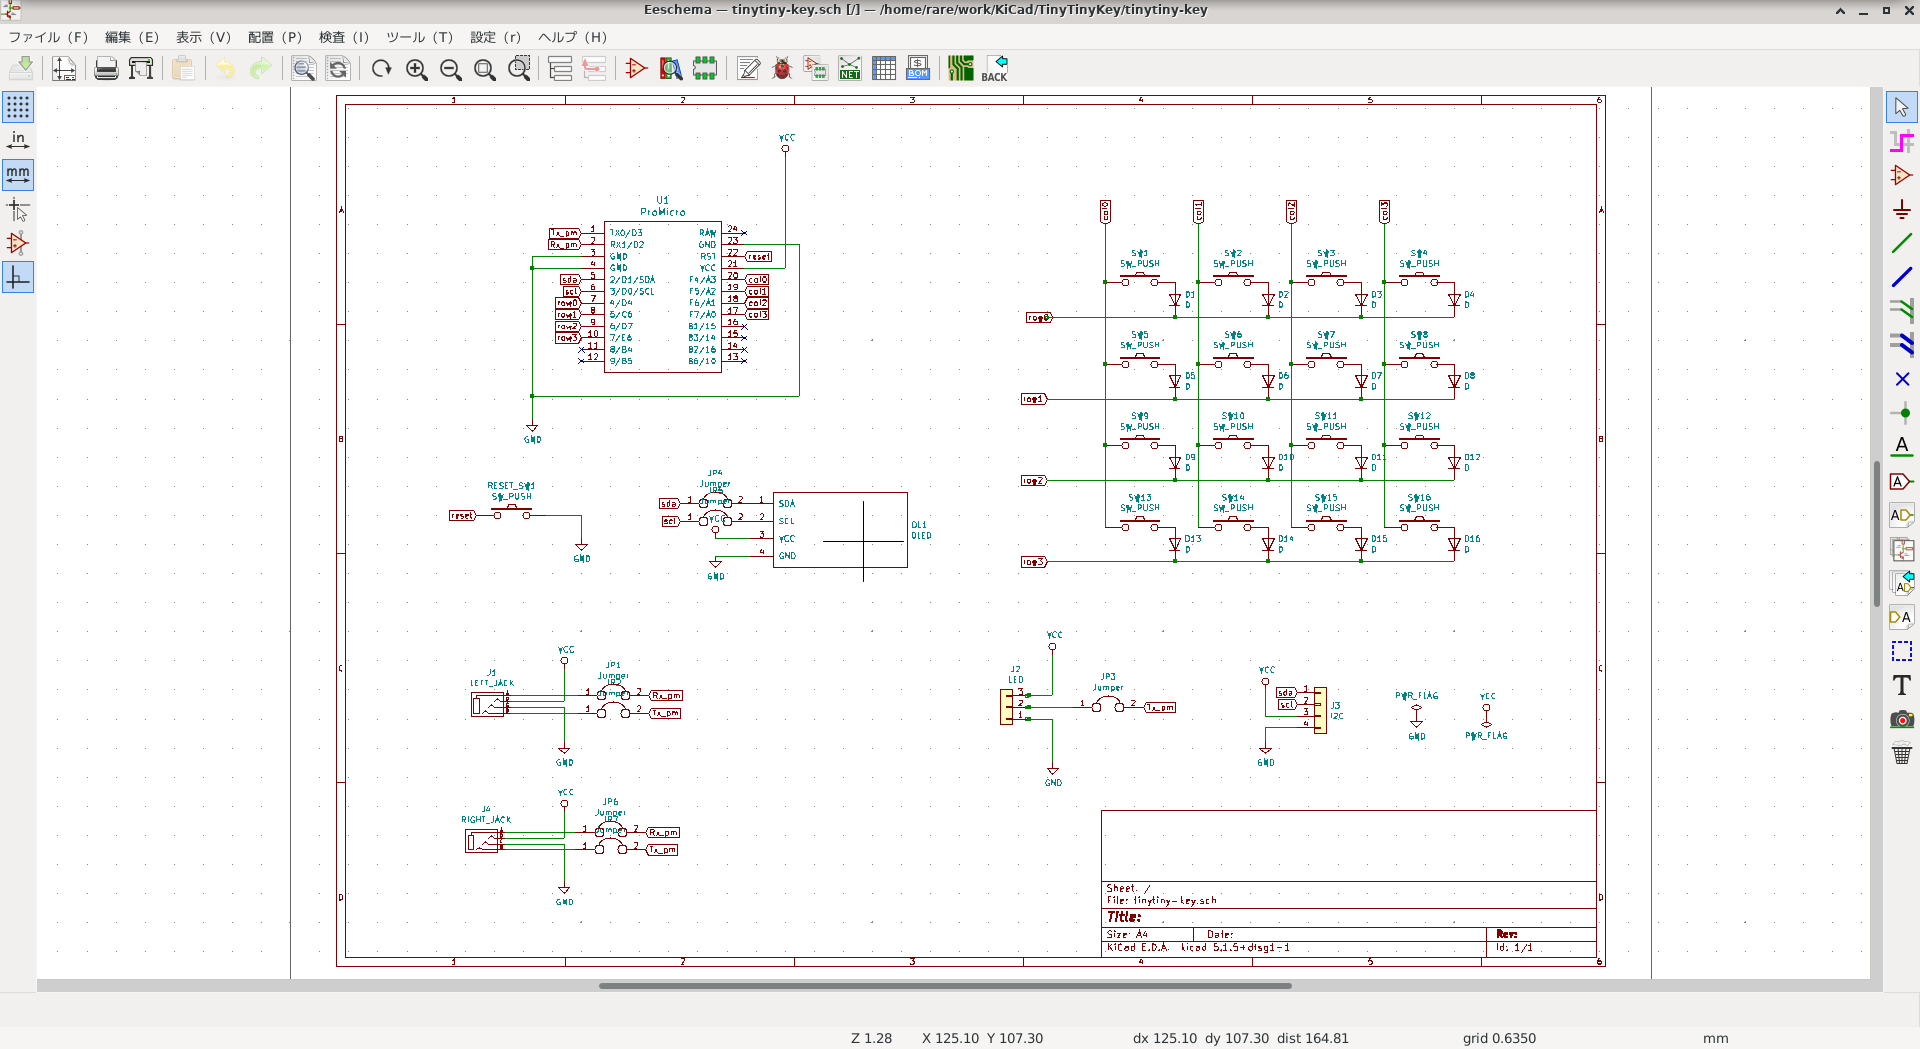
\includegraphics[keepaspectratio,height=4cm]{./img/kicad-schematic.png}
 \end{center}
\end{frame}

\begin{frame}[fragile,t]{PCBの設計 -- 志半ば (4/6)}
 \begin{itemize}
  \item 次にフットプリントを関連付けます
	\begin{itemize}
	 \item フットプリントも先程の場所にライブラリが公開されてます
	 \item 各パーツごとにフットプリントをどれにするか地道に選択していきます
	       \begin{itemize}
		\item Cherry MX / Kailhロープロの両対応のフットプリントもあります
	       \end{itemize}
	\end{itemize}
 \end{itemize}
 \begin{center}
  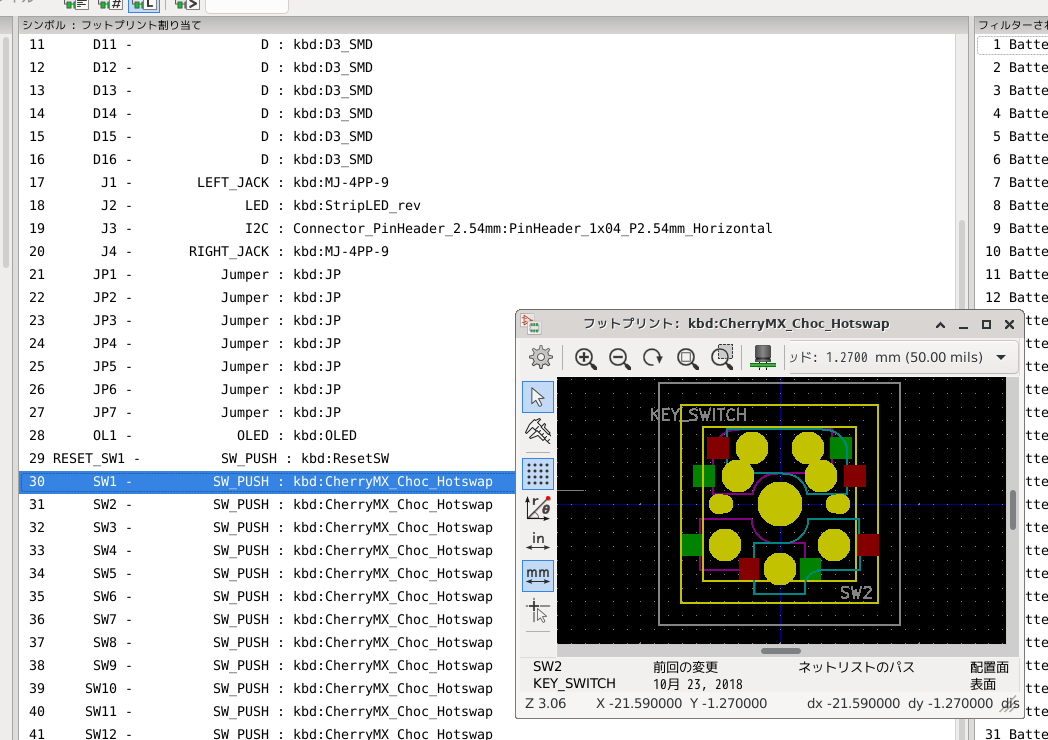
\includegraphics[keepaspectratio,height=4cm]{./img/kicad-footprint.png}
 \end{center}
\end{frame}

\begin{frame}[fragile,t]{PCBの設計 -- 志半ば (5/6)}
 \begin{itemize}
  \item 次にレイアウトをしていきます
	\begin{itemize}
	 \item パーツが干渉しないように注意して……
	 \item 発表者は現状ではここで力尽きてます
	 \item キーのレイアウト用のツールもある
	       \begin{itemize}
		\item \url{http://www.keyboard-layout-editor.com/}
	       \end{itemize}
	\end{itemize}
 \end{itemize}
 \begin{center}
  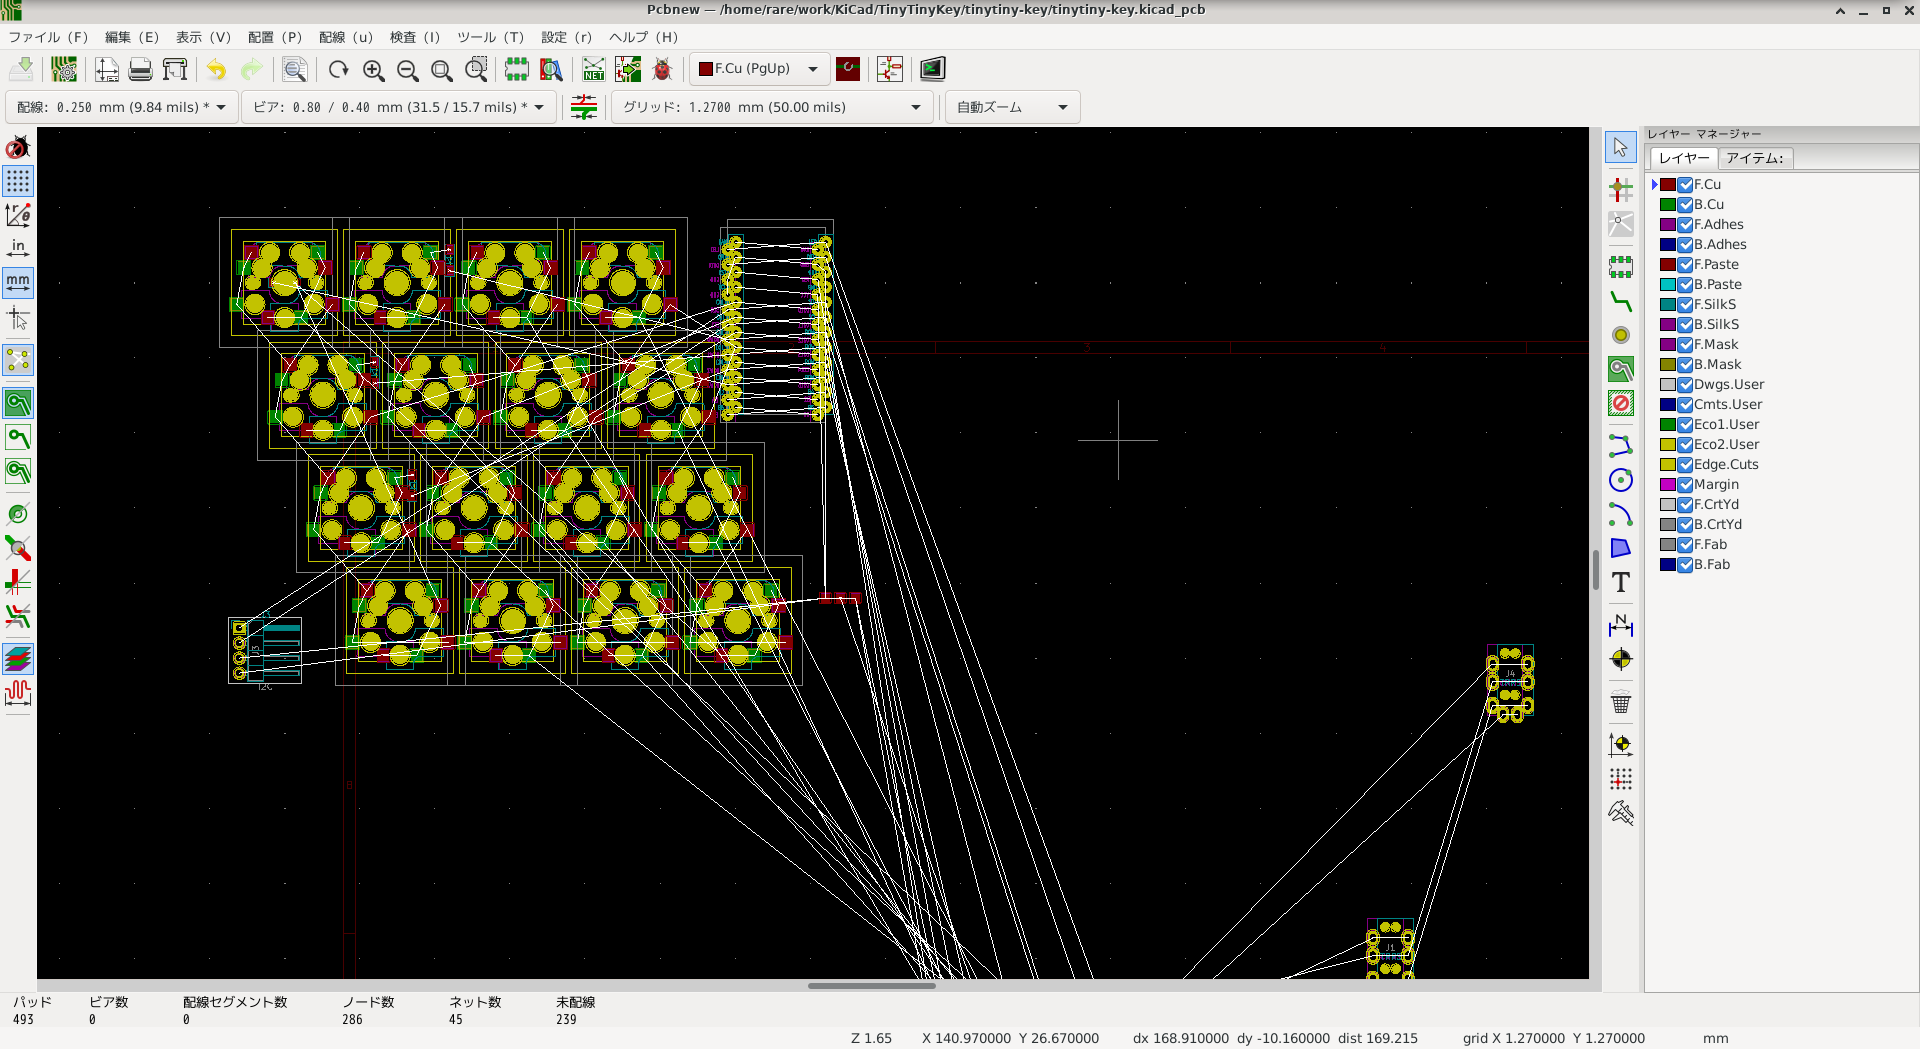
\includegraphics[keepaspectratio,height=4cm]{./img/kicad-layout.png}
 \end{center}
\end{frame}

\begin{frame}[fragile,t]{PCBの設計 -- 志半ば (6/6)}
 \begin{itemize}
  \item この後は……
	\begin{itemize}
	 \item エッジカット線を引く
	 \item スペーサー用の穴をあける
	 \item 配線を実施する(一番大変らしい)
	 \item 必要に応じてケースを作成する
	       \begin{itemize}
		\item アクリル板を加工するのが主流
		\item 最近は3Dプリンタ勢が増えているみたい……
	       \end{itemize}
	\end{itemize}
  \item PCBデータが公開されているキーボードの改変をするという手もある
	\begin{itemize}
	 \item Helix : \url{https://github.com/MakotoKurauchi/helix}
	 \item fortitude60: \url{https://github.com/Pekaso/fortitude60}
	\end{itemize}
 \end{itemize}
\end{frame}

\begin{frame}[fragile,t]{キーボード情報}
 \begin{itemize}
  \item 最後に、どんなところで情報を得るのが良いかご紹介
	\begin{itemize}
	 \item \href{https://yushakobo.jp/}{遊舎工房}
	       \begin{itemize}
		\item 自作キーボード専門店!
		\item 秋葉原訪問の際は是非(どっちかというと末広町のが近い)
	       \end{itemize}
	 \item ミートアップ系
	       \begin{itemize}
		\item \href{https://tenkey.connpass.com/event/150626/}{天下一キーボードわいわい会 Vol.3}
		\item \href{https://selfmade-keyboad-fan-club.connpass.com/event/152614/}{【大阪】自作キーボード作成会}
		\item \href{https://connpass.com/event/132509/}{自作キーボード入門ワークショップ in シリコンハウス}
		\item シリコンハウスさんは最近キットも置きだした
	       \end{itemize}
	 \item Youtube
	       \begin{itemize}
		\item \href{https://www.youtube.com/channel/UCyU1PAGvw_suAyI4wljHmag}{ほぼ週刊キーボードニュース}
	       \end{itemize}
	\end{itemize}
 \end{itemize}
\end{frame}

\begin{frame}[fragile,t]{まとめ(やりなおし)}
 \begin{itemize}
  \item 自作キーボード
	\begin{itemize}
	 \item 分離型とか
	 \item 配列だとかキースイッチについて好みを考える
	 \item 最初はあまり(極端にキーが少ないとか)奇抜なキーボードは避けた方が良い
	 \item 組み立てはチップ(LED/ダイオード)がないキットであればそこまで難しくない
	       \begin{itemize}
		\item 動作確認はマメにしよう(経験者談)
	       \end{itemize}
	 \item キーマップは、結構試行錯誤が必要
	\end{itemize}
  \item PCBからの自作
	\begin{itemize}
	 \item 10cmx10cmでお試しするのがよさそう
	 \item PCBデータの作成にはフリーのKiCadがつかえる
	\end{itemize}
 \end{itemize}
\end{frame}

\takahashi[30]{みなさんも温泉入りませんか?}

\end{document}